\documentclass[
	12pt,
	openright,
	oneside,
	a4paper,
	english,
	brazil
	]{abntex2}

% ---
% PACOTES BÁSICOS
% ---
\usepackage{lmodern}
\usepackage[T1]{fontenc}
\usepackage[utf8]{inputenc}
\usepackage{indentfirst}
\usepackage{color}
\usepackage{graphicx}
\usepackage{microtype}
\usepackage{amsmath}
\usepackage{amssymb}
\usepackage{listings}
\usepackage{xcolor}
\usepackage{url}
\usepackage{booktabs}
\usepackage{float}
\usepackage{subcaption}
\usepackage[alf]{abntex2cite}

% Configuração de código-fonte
\lstset{
  basicstyle=\footnotesize\ttfamily,
  breaklines=true,
  frame=single,
  captionpos=b,
  language=Python,
  keywordstyle=\color{blue},
  commentstyle=\color{gray},
  stringstyle=\color{red},
}

% ---
% INFORMAÇÕES DO TRABALHO
% ---
\titulo{Filtro de Dados e Compressão para Computação em Névoa em IoT na Agricultura Inteligente utilizando Rust e WebAssembly}
\autor{Victor Cobo Figueiro}
\local{Santo André}
\data{2026}
\orientador{Prof. Dr. Carlos Alberto Kamienski}
\instituicao{%
  UNIVERSIDADE FEDERAL DO ABC
  \par
  CMCC -- CENTRO DE MATEMÁTICA, COMPUTAÇÃO E COGNIÇÃO
  \par
  BACHARELADO EM CIÊNCIA DA COMPUTAÇÃO}
\tipotrabalho{Projeto de Graduação em Computação}
\preambulo{Projeto de Graduação em Computação apresentado ao Bacharelado em Ciência da Computação da Universidade Federal do ABC, como requisito parcial para a obtenção do título de Bacharel.}

% ---
% CONFIGURAÇÕES DE APARÊNCIA E CAPA
% ---
\definecolor{blue}{RGB}{41,5,195}
\hypersetup{
    pdftitle={\@title},
    pdfauthor={\@author},
    pdfsubject={\imprimirpreambulo},
    colorlinks=true,
    linkcolor=black,
    citecolor=black,
    urlcolor=black
}

\renewcommand{\imprimircapa}{%
  \begin{capa}%
    \centering
    \vspace*{1cm}
    
\includegraphics[width=4cm]{Ufabc_logo.png} \\
    \vspace{0.5cm}
    {\ABNTEXchapterfont\large\imprimirinstituicao}
    
    \vspace*{\fill}
    
    {\ABNTEXchapterfont\large\imprimirautor}
    
    \vspace*{\fill}
    
    {\ABNTEXchapterfont\bfseries\LARGE\imprimirtitulo}
    
    \vspace*{\fill}
    
    {\large\imprimirlocal}
    \par
    {\large\imprimirdata}
    \vspace*{1cm}
  \end{capa}
}

% ---
% INÍCIO DO DOCUMENTO
% ---
\begin{document}

\selectlanguage{brazil}
\frenchspacing

% ----------------------------------------------------------
% ELEMENTOS PRÉ-TEXTUAIS
% ----------------------------------------------------------
\imprimircapa
\imprimirfolhaderosto

% --- Dedicatória ---
\begin{dedicatoria}
   \vspace*{\fill}
   \centering
   \noindent
   \textit{Dedico este trabalho à minha família pelo apoio incondicional, aos meus colegas de curso pelas noites de estudo compartilhadas, e a todos que enxergam na computação uma ferramenta para transformar a interação humana com o meio ambiente.}
   \vspace*{\fill}
\end{dedicatoria}

% --- Agradecimentos ---
\begin{agradecimentos}
Agradeço primeiramente ao meu orientador, Prof. Dr. Carlos Alberto Kamienski, pelo suporte técnico, paciência e pelas valiosas discussões acadêmicas ao longo do desenvolvimento deste projeto. Agradeço profundamente aos meus pais pelo apoio incondicional, amor e sacrifícios que tornaram esta conquista possível. Aos meus grandes amigos Leandro Diomar e Carlos Quintino, agradeço pelo companheirismo, incentivo constante e pelas noites de estudo compartilhadas durante toda esta jornada acadêmica. Por fim, agradeço à Universidade Federal do ABC pelo ensino público de excelência e a todos os professores que contribuíram para minha formação científica.
\end{agradecimentos}

% --- Epígrafe ---
\begin{epigrafe}
    \vspace*{\fill}
	\begin{flushright}
		\textit{``A simplicidade é um grande pré-requisito para a confiabilidade.''\\
		(Edsger W. Dijkstra)}
	\end{flushright}
\end{epigrafe}

% --- Resumo ---
\begin{resumo}
A agricultura inteligente é uma das principais fronteiras da Internet das Coisas (IoT), exigindo o monitoramento de variáveis físicas contínuas em ambientes remotos. Contudo, a transmissão em tempo real de grandes volumes de dados de sensores para a nuvem por canais de baixa potência e banda restrita (como LoRaWAN) gera alta latência, congestionamento e rápido esgotamento energético dos dispositivos. Como continuação direta e implementação prática da pesquisa teórica proposta por Ribeiro Junior et al. \cite{ribeiro2020nearest}, este trabalho propõe e avalia um ecossistema de computação em névoa baseado em Rust e WebAssembly (WASM) para realizar filtragem e compressão de dados na borda da rede. Utilizando o algoritmo de classificação $k$-Vizinhos Mais Próximos ($k$NN, com $k=3$) adaptado para as condições agronômicas de cultivo do tomateiro, o sistema converte medidas físicas contínuas de temperatura e umidade em status discretos de um caractere, os quais são posteriormente comprimidos via Run Length Encoding (RLE). Para a validação estatística, implementou-se um gerador de dados estocásticos via Estimativa de Densidade por Kernel (KDE) e Transformada de Box-Muller nativamente em Rust/WASM. Os experimentos compararam a base original (\texttt{entrada.csv}, com 44.023 registros) e amostras sintéticas de 40.000 pontos em três execuções independentes. O gerador em Rust demonstrou altíssima fidelidade estatística, validada pelo teste de Kolmogorov-Smirnov (p-valor de $0,1385$ para temperatura e $0,8974$ para umidade) e pelo desvio de correlação de Pearson de apenas $0,0033$. Os resultados mostraram que o kNN isolado alcança $97,84\%$ de redução de volume de dados (reduzindo a base para 40 KB), superando a combinação kNN+RLE ($96,32\%$, ou 68 KB). Isso revela a ineficiência do RLE em alfabetos curtos de caractere único frente à variabilidade natural de alta frequência dos sensores físicos, fornecendo diretrizes de projeto cruciais para arquiteturas de IoT na névoa.

\textbf{Palavras-chave}: Computação em Névoa. Internet das Coisas (IoT). Agricultura Inteligente. Rust. WebAssembly. WasmEdge. Compressão de Dados.
\end{resumo}

% --- Abstract ---
\begin{resumo}[Abstract]
\begin{otherlanguage*}{english}
Smart agriculture stands as one of the primary frontiers for the Internet of Things (IoT), requiring continuous monitoring of environmental variables in remote areas. However, streaming large volumes of raw sensor data directly to the cloud over low-power, narrow-bandwidth channels (such as LoRaWAN) causes network congestion, latency, and rapid battery depletion. As a direct continuation and practical implementation of the theoretical research proposed by Ribeiro Junior et al. \cite{ribeiro2020nearest}, this work proposes and evaluates a fog computing ecosystem built with Rust and WebAssembly (WASM) to perform data filtering and compression at the network edge. Using a $k$-Nearest Neighbors classification algorithm ($k$NN, with $k=3$) tailored to tomato agronomic status, the system maps continuous temperature and humidity readings into single-character discrete labels, which are compressed using Run Length Encoding (RLE). For validation, an offline stochastic data generator was developed natively in Rust/WASM using Kernel Density Estimation (KDE) and the Box-Muller transform. Experiments compared the original dataset (\texttt{entrada.csv}, 44,023 records) with synthetic samples of 40,000 points across three independent runs. The Rust generator achieved high statistical fidelity, validated by the Kolmogorov-Smirnov test (p-value of $0.1385$ for temperature and $0.8974$ for humidity) and a Pearson correlation deviation of just $0.0033$. Results showed that standalone $k$NN achieves a $97.84\%$ data reduction (shrinking the payload to 40 KB), outperforming the combined $k$NN+RLE approach ($96.32\%$, or 68 KB). This highlights the inefficiency of RLE when applied to a single-character alphabet under high-frequency physical sensor fluctuations, providing critical design guidelines for fog-based IoT architectures.

\vspace{\onelineskip}
\noindent
\textbf{Keywords}: Fog Computing. Internet of Things (IoT). Smart Agriculture. Rust. WebAssembly. WasmEdge. Data Compression.
\end{otherlanguage*}
\end{resumo}

% --- Listas ---
\pdfbookmark[0]{\listfigurename}{lof}
\listoffigures*
\cleardoublepage

\pdfbookmark[0]{\listtablename}{lot}
\listoftables*
\cleardoublepage

% --- Sumário ---
\pdfbookmark[0]{\contentsname}{toc}
\tableofcontents*
\cleardoublepage

% ----------------------------------------------------------
% ELEMENTOS TEXTUAIS
% ----------------------------------------------------------
\textual

% ==========================================================
\chapter{INTRODUÇÃO}
% ==========================================================

A Internet das Coisas (IoT) revolucionou a agricultura de precisão, permitindo que sensores coletem continuamente variáveis ambientais como temperatura, umidade, luminosidade e umidade do solo. Na agricultura inteligente, o monitoramento em tempo real dessas grandezas é vital para otimizar a produtividade e a saúde das plantações. No entanto, a arquitetura tradicional que centraliza a coleta de dados e os envia diretamente à nuvem enfrenta graves gargalos operacionais.

Sensores implantados no campo operam sob fortes restrições de energia e dependem de redes de comunicação sem fio de baixa potência e longo alcance (LPWAN), como LoRaWAN, que operam com taxas de transmissão extremamente baixas (tipicamente entre 292 bps e 50 kbps) e limitações rígidas de ciclo de trabalho (\textit{duty cycle}) \cite{adelantado2017lorawan}. O envio ininterrupto de dados brutos gera alto consumo de bateria nos nós sensores e congestionamento de rede no gateway.

Nesse cenário, a computação em névoa (\textit{fog computing}) atua como uma camada intermediária entre os dispositivos sensores de borda e os servidores em nuvem. Ao transferir capacidade computacional de processamento e tomada de decisão para os gateways locais, torna-se possível aplicar algoritmos de filtragem de dados e compressão antes da transmissão WAN. Desta forma, envia-se apenas informação relevante para a nuvem, economizando largura de banda e prolongando a vida útil das baterias dos nós de borda.

Este trabalho apresenta-se como uma continuação direta e evolução prática da pesquisa pioneira desenvolvida por Ribeiro Junior et al. \cite{ribeiro2020nearest}, transpondo e testando seus modelos teóricos em uma arquitetura executável e de alto desempenho na névoa.

\section{PROBLEMA DE PESQUISA}

A filtragem de dados na névoa exige um ambiente de execução leve, portável e seguro para rodar códigos de terceiros nos gateways de borda. Máquinas virtuais pesadas ou contêineres tradicionais (como Docker) demandam muitos recursos computacionais, tornando-se inviáveis para os hardwares limitados comuns na névoa. Além disso, linguagens tradicionais de script (como Python) carecem do desempenho e eficiência necessários, enquanto linguagens compiladas nativas (como C/C++) apresentam riscos severos de segurança de memória.

A pesquisa original de Ribeiro Junior et al. \cite{ribeiro2020nearest} propôs o uso de $k$-Vizinhos Mais Próximos ($k$NN) e Run Length Encoding (RLE) em gateways para reduzir a taxa de transmissão em aplicações agrícolas. Contudo, a viabilização prática desse modelo em sistemas de produção exige responder à seguinte questão: \textit{Como implementar e validar um ecossistema seguro, portável e de alto desempenho para filtragem e compressão de dados agrícolas na borda, utilizando modernas tecnologias de compilação como Rust e WebAssembly, e como garantir a estabilidade e a validade estatística desse processamento em cenários off-line?}

\section{OBJETIVOS}

\subsection{Objetivo Geral}

Propor, implementar e validar um framework fim-a-fim de computação em névoa que realiza filtragem de dados agronômicos por meio de classificação $k$NN e compressão RLE, compilado para WebAssembly (WASM) a partir de Rust e executado no ambiente de alto desempenho WasmEdge.

\subsection{Objetivos Específicos}

\begin{itemize}
    \item Implementar o classificador $k$NN ($k=3$) para classificar dados de sensores em 11 classes de sanidade do tomateiro;
    \item Desenvolver o codificador RLE em Rust para comprimir sequências de classes resultantes do kNN;
    \item Desenvolver um módulo de simulação estocástica de dados nativo em Rust que implementa Estimativa de Densidade por Kernel (KDE) e Transformada de Box-Muller para ambiente WASM/WASI;
    \item Validar estatisticamente a fidelidade do gerador estocástico contra a base de dados reais de sensores (\texttt{entrada.csv}) por meio de testes de Kolmogorov-Smirnov (KS-test) e correlação de Pearson;
    \item Avaliar comparativamente a eficiência de compressão obtida com kNN isolado e kNN+RLE sob diferentes tamanhos de lote de processamento.
\end{itemize}

\section{JUSTIFICATIVA}

A transposição de algoritmos de processamento de dados para a névoa usando a linguagem Rust e o ambiente WebAssembly justifica-se por razões tecnológicas e práticas fundamentais:

\textbf{Desempenho e Segurança}: Rust garante segurança de memória sem a necessidade de um coletor de lixo (\textit{garbage collector}), entregando eficiência equivalente a C/C++ sem o risco de falhas catastróficas (\textit{buffer overflows}, vazamento de memória).

\textbf{Otimização com WebAssembly e WasmEdge}: Rust funciona de maneira ideal ao ser compilado para alvos WebAssembly (WASM), gerando bytecode portável de alta segurança executado quase à velocidade nativa. A execução sob o runtime \textbf{WasmEdge} expande as limitações tradicionais do padrão WASI ao fornecer suporte nativo para soquetes de rede e chamadas HTTP de forma direta de dentro do sandbox isolado. Isso viabiliza que o gateway de névoa faça o upload dos pacotes de dados classificados e comprimidos diretamente para os servidores de nuvem de forma assíncrona, descartando a dependência de processos nativos adicionais e garantindo isolamento estrito de segurança.

\textbf{Economia de Infraestrutura}: A redução sistemática do tamanho dos pacotes e da frequência de envio viabiliza na prática a implantação de um número maior de sensores sob a mesma infraestrutura LoRaWAN existente.

\textbf{Validação Estatística com Dados Sintéticos}: A capacidade de gerar dados sintéticos estatisticamente idênticos permite testar de forma robusta e exaustiva novos algoritmos e configurações de rede off-line, sem a necessidade de dispendiosas campanhas de campo para coleta contínua.

\section{DISCIPLINAS FORMADORAS DO PROJETO}

O desenvolvimento do projeto utilizou conceitos de diversas áreas de conhecimento da Ciência da Computação da UFABC, conforme detalhado na Tabela~\ref{tab:disciplinas}.

\begin{table}[H]
\centering
\caption{Disciplinas do BCC/UFABC e sua contribuição ao projeto}
\label{tab:disciplinas}
\resizebox{\textwidth}{!}{%
\begin{tabular}{|p{5.5cm}|p{3.5cm}|p{7.5cm}|}
\hline
\textbf{Disciplina} & \textbf{Código} & \textbf{Contribuição ao Projeto} \\ \hline

Inteligência Artificial & MCTA014-15 &
Fundamentação de classificadores supervisionados para a concepção e parametrização do algoritmo $k$NN. \\ \hline

Sistemas Distribuídos & MCTA025-13 &
Comunicação cliente-servidor e arquitetura de dados IoT na passagem de dados de sensores do Thing para a Névoa e para a Nuvem. \\ \hline

Redes de Computadores & MCTA024-13 &
Conhecimentos sobre protocolos de comunicação de baixo consumo e restrições de transmissão em canais sem fio de longa distância. \\ \hline

Compiladores & MCTA009-17 &
Compreensão da geração de representação intermediária e otimização de código necessária para compilar código Rust em bytecode WebAssembly. \\ \hline

Algoritmos e Estruturas de Dados II & MCTA002-17 &
Estruturas de representação na memória para busca de vizinhos mais próximos e indexação de buffer de dados temporais para compressão RLE. \\ \hline

\end{tabular}%
}
\fonte{O Autor (2026)}
\end{table}

Todo o código-fonte desenvolvido para este projeto, incluindo os módulos do ecossistema distribuído em Rust e os scripts auxiliares em Python, está disponível publicamente no GitHub no repositório \href{https://github.com/v-cobof/pgc-rust}{\texttt{https://github.com/v-cobof/pgc-rust}}.

\section{ORGANIZAÇÃO DO TEXTO}

Este trabalho está estruturado da seguinte forma: o Capítulo~\ref{cap:referencial} apresenta o referencial teórico cobrindo as tecnologias Rust, WebAssembly, kNN, RLE, o gerador estocástico e a revisão da literatura de base; o Capítulo~\ref{cap:desenvolvimento} descreve a arquitetura e implementação dos componentes; o Capítulo~\ref{cap:metodologia} apresenta a metodologia de teste e o plano de validação; o Capítulo~\ref{cap:resultados} discute os resultados obtidos, acompanhados das análises estatísticas e dos gráficos; e o Capítulo~\ref{cap:conclusao} resume as principais conclusões e propostas para trabalhos futuros.

% ==========================================================
\chapter{REFERENCIAL TEÓRICO}
\label{cap:referencial}
% ==========================================================

\section{Computação em Névoa (Fog Computing)}

A computação em névoa (\textit{Fog Computing}) estende os recursos computacionais, de armazenamento e de rede da computação em nuvem para a proximidade física dos dispositivos de borda na Internet das Coisas (IoT) \cite{bonomi2012fog}. O paradigma surge como uma camada arquitetural intermediária necessária para lidar com o crescimento exponencial de sensores físicos gerando dados em alta frequência. 

Nas arquiteturas de IoT convencionais, o sensoriamento contínuo depende de protocolos de transporte leves para comunicação com a nuvem, tais como o MQTT (\textit{Message Queuing Telemetry Transport}) ou o CoAP (\textit{Constrained Application Protocol}) \cite{alfuqaha2015iot}. No entanto, mesmo com o uso de payloads enxutos baseados nesses protocolos, a transmissão ininterrupta de dados brutos e ruidosos (por exemplo, leituras decimais de temperatura e umidade a cada poucos segundos) gera gargalos severos de rede, especialmente em áreas agrícolas remotas operando sob conexões sem fio instáveis ou satelitais de alto custo.

Ao contrário da infraestrutura centralizada da nuvem, a névoa caracteriza-se por sua distribuição geográfica descentralizada, suporte à mobilidade de nós, baixa latência de comunicação e forte dependência de conexões de rádio locais \cite{buyya2018fog}. Em sistemas agrícolas modernos, os nós de névoa — representados por computadores de placa única como Raspberry Pi ou gateways industriais — processam dados de sensores de campo locally, filtrando ruídos, executando lógica analítica e encaminhando apenas informações consolidadas ou alarmes para a nuvem. Isso reduz significativamente a dependência de conexões WAN de alto custo ou restritas (como satélite ou celular) e otimiza o uso de banda larga de rede.

\section{IoT-Cloud Continuum (IoTinuum)}

O conceito de contínuo IoT-Nuvem (\textit{IoT-Cloud Continuum}), também designado na literatura técnica por \textit{IoTinuum}, representa uma quebra de paradigma na infraestrutura tradicional de sistemas da Internet das Coisas (IoT). Em vez de modelar a rede em camadas computacionais isoladas e silos de comunicação monolíticos, o contínuo propõe uma integração sem costuras, orquestrada de ponta a ponta, que se estende dos dispositivos mais básicos e periféricos até os servidores corporativos centralizados na nuvem \cite{kamienski2017iotinuum}.

Para estruturar e viabilizar este contínuo, a literatura descreve uma arquitetura de referência tipicamente dividida em três fases ou camadas fundamentais \cite{naha2018fog, puliafito2019mobility}:
\begin{enumerate}
    \item \textbf{Things / Dispositivos Físicos (Fase de Aquisição)}: Representa a camada de sensoriamento de borda extrema. É composta por nós de sensores (ex: DHT22, termopares) e microcontroladores de baixíssimo custo de processamento, cuja função prioritária é coletar e digitalizar grandezas físicas (temperatura, umidade, pressão) do ambiente agrícola inteligente. Nesta camada, a capacidade de memória RAM e de processamento é tão severamente restrita que tarefas complexas de filtragem não podem ser executadas localmente;
    \item \textbf{Edge e Fog Computing (Fase de Pré-processamento e Filtragem)}: Camada intermediária que reside na rede local. Os nós de névoa (\textit{fog nodes}), como gateways de comunicação industrial, Raspberry Pi ou servidores locais, atuam como pontes ativas entre o campo físico e a rede WAN. Estes nós concentram dados de múltiplos sensores locais, executam algoritmos inteligentes de classificação (como $k$NN) e encoders de compactação (como RLE) para extrair o status agronômico do ambiente e comprimir redundâncias antes do envio para a Internet;
    \item \textbf{Cloud Computing (Fase Analítica Global e Persistência)}: Camada superior centralizada de alta disponibilidade e capacidade de processamento (ex: clusters AWS ou Google Cloud). Na nuvem, os dados comprimidos são decodificados, indexados em bancos de dados históricos de longo prazo, apresentados aos produtores em painéis gráficos interativos e utilizados para treinar algoritmos de aprendizado de máquina globais.
\end{enumerate}

Um dos maiores desafios científicos no gerenciamento do contínuo consiste na orquestração dinâmica dessas camadas distribuídas. Frameworks de orquestração consolidados na nuvem (como Kubernetes ou suas variantes voltadas à borda como KubeEdge) impõem uma sobrecarga de CPU, memória RAM e armazenamento que inviabiliza sua implantação em pequenos gateways embarcados locais \cite{pfandzelter2021orchestration}. O ecossistema do contínuo demanda, portanto, uma arquitetura de execução de microsserviços muito mais leve e flexível, capaz de migrar código compilado de maneira rápida e segura entre os diferentes nós de hardware do \textit{IoTinuum} sem a necessidade de manter sistemas operacionais virtuais pesados.

\section{Rust e WebAssembly (WASM): Os Encoders do IoTinuum}

Para que a migração de tarefas seja viável na prática ao longo do contínuo heterogêneo do \textit{IoTinuum}, a engenharia de software exige um ecossistema que combine eficiência de recursos com isolamento e portabilidade. O núcleo deste trabalho baseia-se na união da linguagem de programação Rust com o bytecode do WebAssembly (WASM), atuando como o elemento catalisador da computação portátil na névoa.

\subsection{Linguagem Rust}

Rust é uma linguagem de sistemas focada em segurança de memória, velocidade de execução e concorrência eficiente \cite{matsakis2014rust}. Por meio de seu inovador sistema de checagem de regras de empréstimo e tempo de vida de dados (\textit{borrow checker}), a linguagem garante o controle estrito sobre alocações de memória diretamente em tempo de compilação, eliminando a necessidade de um coletor de lixo (\textit{garbage collector}). 

Esta característica traduz-se em binários com consumo de memória extremamente baixo e tempo de resposta previsível. Rust é a linguagem ideal para codificar algoritmos analíticos em nós de névoa e sensores de campo de baixa potência, gerando o máximo de eficiência energética.

\subsection{WebAssembly (WASM) e WASI}

O WebAssembly (WASM) é um formato de instrução binária de baixo nível projetado para ser executado em uma máquina virtual baseada em pilha com isolamento estrito (\textit{sandboxing}) \cite{haas2017wasm}. Embora originalmente concebido para navegadores web, o WASM expandiu-se rapidamente para cenários de computação de borda e névoa devido à introdução da \textit{WebAssembly System Interface} (WASI), que padroniza o acesso seguro a recursos do sistema operacional hospedeiro.

Ao contrário de ambientes tradicionais baseados na Máquina Virtual Java (JVM) — que impõem um consumo massivo de memória em tempo de execução — ou de contêineres Docker — que exigem o isolamento pesado a nível de kernel e imagens de dezenas de megabytes —, o bytecode WASM é executado a velocidades quase nativas (tipicamente com desvio de apenas 1,1x a 1,5x o desempenho do código compilado diretamente para a máquina nativa) utilizando compilação JIT (\textit{Just-In-Time}) e AOT (\textit{Ahead-Of-Time}) em ambientes constritos de hardware \cite{varia2021wasm}.

O WASM apresenta vantagens tecnológicas cruciais frente à virtualização tradicional baseada em contêineres Docker para a computação no \textit{IoTinuum} \cite{guan2022wasm}:
\begin{itemize}
    \item \textbf{Portabilidade de Bytecode Universal}: O código compilado para WASM é independente de arquitetura de CPU (ISA-neutral). O mesmo arquivo binário compilado com o target \texttt{wasm32-wasip1} executa sem qualquer modificação em processadores ARM32/ARM64 de gateways locais ou em arquiteturas x86\_64 em datacenters na nuvem, desde que haja um interpretador de bytecode disponível;
    \item \textbf{Inicialização em Microsegundos (Cold Start zero)}: Enquanto contêineres Docker tradicionais necessitam de segundos para iniciar o sistema de arquivos virtualizado e carregar bibliotecas compartilhadas, instâncias WASM são instanciadas em escalas de microsegundos, permitindo que nós sensores entrem em modo de economia de energia e iniciem o processamento instantaneamente ao detectar novos dados;
    \item \textbf{Segurança e Isolamento por Sandbox}: O runtime WASM isola completamente a aplicação em memória. O acesso do bytecode a arquivos, rede ou temporizadores é bloqueado por padrão e deve ser explicitamente fornecido no momento da instanciação da máquina virtual por meio de capabilidades configuradas pelo hospedeiro;
    \item \textbf{Footprint Mínimo de Memória e Armazenamento}: Módulos WASM ocupam apenas algumas dezenas de kilobytes, o que otimiza sua distribuição na rede rural e possibilita executar centenas de sandboxes concorrentes em dispositivos embarcados com menos de 512 MB de RAM.
\end{itemize}

\subsection{WasmEdge Runtime}

O WasmEdge é um ambiente de execução (runtime) de WebAssembly de alto desempenho, com suporte a compilações JIT (\textit{Just-In-Time}) e AOT (\textit{Ahead-Of-Time}) \cite{wasmedge2023}. Desenvolvido sob a governança da CNCF, ele destaca-se no ecossistema de borda e névoa por estender a especificação WASI básica com capabilidades avançadas de rede. 

Uma vez que a especificação padrão WASI clássica carece de primitivas nativas de comunicação por rede TCP/UDP, o WasmEdge preenche esta lacuna por meio de APIs que expõem soquetes de rede ao sandbox de maneira segura. Isso possibilita ao ecossistema do processador e do receptor em Rust rodar servidores HTTP assíncronos complexos e realizar chamadas de rede REST diretamente de dentro da máquina virtual WASM na névoa, unindo a segurança do sandbox com a capacidade de integração do \textit{IoTinuum}.

\section{Algoritmo dos k-Vizinhos Mais Próximos (kNN)}

O $k$NN é um algoritmo de aprendizado supervisionado não-paramétrico. O princípio consiste em classificar um novo ponto no espaço tridimensional ou bidimensional a partir do voto majoritário dos seus $k$ vizinhos mais próximos no conjunto de treino.

Para que variáveis físicas com ordens de grandeza distintas (como temperatura em ${}^\circ\text{C}$ e umidade em $\%$) tenham o mesmo peso no cálculo das distâncias, aplica-se a normalização Min-Max dos dados para o intervalo $[0, 1]$ com base nos limites $x_{min}$ e $x_{max}$ obtidos a priori:
\begin{equation}
x_{norm} = \frac{x - x_{min}}{x_{max} - x_{min}}
\end{equation}

A distância Euclidiana entre um vetor de leitura de sensor $P = (T_p, H_p)$ e um ponto do conjunto de treinamento $Q = (T_q, H_q)$ no espaço normalizado bidimensional é dada por:
\begin{equation}
d(P, Q) = \sqrt{(T_{p,norm} - T_{q,norm})^2 + (H_{p,norm} - H_{q,norm})^2}
\end{equation}

O algoritmo seleciona os $k$ registros de treinamento com as menores distâncias $d$ e realiza uma votação majoritária para determinar a classe agronômica a ser associada à nova leitura física.

\section{Compressão Run Length Encoding (RLE)}

A codificação de comprimento de corrida (RLE) é um método simples de compressão de dados sem perdas (\textit{lossless}), ideal para sequências com repetições frequentes de símbolos idênticos. O algoritmo substitui sequências contíguas de um mesmo caractere por um par constituído pelo número de ocorrências e o próprio caractere (exemplo: a cadeia \texttt{AAAAABBB} é representada por \texttt{5A3B}). 

Em dados agrícolas classificados por kNN, a redundância temporal é elevada, uma vez que a temperatura e a umidade mudam lentamente, gerando longas corridas consecutivas do mesmo status agronômico (por exemplo, várias horas consecutivas no estado "Optimal").

\section{Geração Estocástica via KDE e Box-Muller}

No contexto deste projeto, a Estimativa de Densidade por Kernel (KDE) e a Transformada de Box-Muller foram utilizadas para conceber e implementar um \textbf{gerador estocástico off-line de dados de sensores} integrado diretamente no processador em Rust. Em cenários de IoT agrícola, a realização de campanhas contínuas de campo para coleta física de sensores pode ser financeiramente inviável ou limitada no tempo. Com a incorporação do gerador KDE, o gateway de névoa é capaz de sintetizar grandes conjuntos de dados (como as séries de 40.000 pontos avaliadas nos experimentos) estatisticamente consistentes com as leituras físicas originais (\texttt{entrada.csv}). A transformada de Box-Muller é o mecanismo que viabiliza essa geração estocástica de forma autônoma de dentro do \textit{sandbox} isolado do WebAssembly (WASI), onde os geradores de números aleatórios nativos do sistema operacional hospedeiro são inacessíveis ou severamente restritos. Essa emulação de alta fidelidade permite realizar baterias de testes experimentais off-line, avaliar o comportamento dinâmico de rede e verificar a eficiência dos algoritmos de classificação e compressão sob cargas realistas de sensores sem a necessidade de acoplamento físico com o hardware no gateway durante fases de validação.

\subsection{Estimativa de Densidade por Kernel (KDE)}

O KDE é um método não-paramétrico para estimar a função de densidade de probabilidade (PDF) de uma variável aleatória contínua multivariada \cite{silverman1986kde}. Dada uma amostra real $\{X_1, X_2, \dots, X_n\}$ extraída da base física, o estimador de densidade por kernel em $d$ dimensões é definido como:
\begin{equation}
\hat{f}(x) = \frac{1}{n h^d} \sum_{i=1}^n K\left(\frac{x - X_i}{h}\right)
\end{equation}
onde $h > 0$ é a largura de banda (\textit{bandwidth}) e $K(u)$ é a função de kernel gaussiano normal multivariado.

Para gerar um novo ponto sintético $x_{sint} = (T_{sint}, H_{sint})$ a partir do KDE:
\begin{enumerate}
    \item Seleciona-se uniformemente ao acaso um ponto base $X_i = (T_i, H_i)$ do conjunto de dados reais (\texttt{entrada.csv});
    \item Adiciona-se ruído normal independente de média $0$ e desvio padrão igual à largura de banda $h = 0.5$ em cada dimensão:
    \begin{align}
    T_{sint} &= T_i + Z_1 \cdot h \\
    H_{sint} &= H_i + Z_2 \cdot h
    \end{align}
    onde $Z_1, Z_2 \sim \mathcal{N}(0, 1)$ são variáveis aleatórias normais padrão independentes.
\end{enumerate}

\subsection{Transformada de Box-Muller}

A geração de variáveis normais padrão $Z \sim \mathcal{N}(0,1)$ em Rust dentro do sandbox WebAssembly (WASI) requer um algoritmo autossuficiente e determinístico. A transformada de Box-Muller \cite{box1958muller} converte duas variáveis pseudo-aleatórias mutuamente independentes distribuídas uniformemente no intervalo aberto $(0, 1]$, denotadas por $U_1$ e $U_2$, em duas variáveis normais padrão independentes:
\begin{align}
Z_0 &= \sqrt{-2 \ln(U_1)} \cdot \cos(2\pi U_2) \\
Z_1 &= \sqrt{-2 \ln(U_1)} \cdot \sin(2\pi U_2)
\end{align}
Esse método permite gerar o ruído estocástico gaussiano do KDE de forma exata e rápida sem recorrer a bibliotecas de sistema operacional ausentes no sandbox do WASM.

\section{Métodos de Validação Estatística}

Para validar cientificamente a fidelidade dos dados sintéticos gerados pelo processador em relação às leituras originais dos sensores físicos, empregam-se duas abordagens estatísticas complementares: o teste de Kolmogorov-Smirnov (KS) e o coeficiente de correlação de Pearson.

\subsection{Teste de Kolmogorov-Smirnov (KS) de Duas Amostras}

O teste de Kolmogorov-Smirnov (KS) de duas amostras é um teste estatístico não-paramétrico utilizado para comparar se duas distribuições empíricas contínuas provêm da mesma distribuição de probabilidade populacional contínua \cite{massey1951ks}. A principal vantagem deste teste é que ele não assume nenhuma distribuição a priori (como a normalidade) para as variáveis analisadas, sendo amplamente aplicável a qualquer tipo de distribuição contínua.

Dadas duas amostras independentes $X = \{X_1, X_2, \dots, X_n\}$ e $Y = \{Y_1, Y_2, \dots, Y_m\}$ de tamanhos $n$ e $m$, suas funções de distribuição acumulada empírica (ECDF - \textit{Empirical Cumulative Distribution Function}) são definidas, respectivamente, por:
\begin{align}
F_{1,n}(t) &= \frac{1}{n} \sum_{i=1}^n \mathbb{I}_{X_i \leq t} \\
F_{2,m}(t) &= \frac{1}{m} \sum_{j=1}^m \mathbb{I}_{Y_j \leq t}
\end{align}
onde $\mathbb{I}_{A}$ é a função indicadora, assumindo o valor 1 se a condição $A$ for verdadeira e 0 caso contrário.

A estatística de teste de Kolmogorov-Smirnov, denotada por $D$, quantifica a distância máxima vertical absoluta entre as duas ECDFs:
\begin{equation}
D = \sup_t |F_{1,n}(t) - F_{2,m}(t)|
\end{equation}

Geometricamente, a estatística $D$ representa o supremo da diferença absoluta entre as trajetórias das duas funções acumuladas empíricas. Devido a essa definição, o teste KS é sensível a qualquer diferença de comportamento entre as duas distribuições, incluindo desvios de localização (média), dispersão (variância), assimetria (\textit{skewness}) ou curtose.

A hipótese nula ($H_0$) assume que ambas as amostras são extraídas da mesma distribuição populacional contínua ($F_1(t) = F_2(t)$ para todo $t$), enquanto a hipótese alternativa ($H_1$) assume que as distribuições são distintas. Rejeita-se $H_0$ a um nível de significância $\alpha$ se a estatística de teste calculada $D$ for superior a um valor crítico limite $d_{\alpha}$. Para amostras de tamanho suficientemente grande ($n, m > 30$), o valor crítico aproximado pode ser determinado assintoticamente por:
\begin{equation}
d_{\alpha} = c(\alpha) \sqrt{\frac{n + m}{n \cdot m}}
\end{equation}
onde o coeficiente $c(\alpha)$ é derivado da distribuição limite de Kolmogorov. Para os níveis de significância usuais de $\alpha = 0,10$, $\alpha = 0,05$ e $\alpha = 0,01$, os valores de $c(\alpha)$ são dados aproximadamente por $1,22$, $1,36$ e $1,63$, respectivamente.

O p-valor correspondente expressa a probabilidade de obter uma estatística de teste pelo menos tão extrema quanto a estatística calculada sob a suposição de que a hipótese nula seja verdadeira. Em termos práticos de teste, se o p-valor for maior que o nível de significância adotado ($\alpha = 0,05$), não se rejeita a hipótese nula $H_0$. No contexto da validação do simulador estocástico desenvolvido em Rust, isso implica que as distribuições geradas sinteticamente e as distribuições físicas reais coletadas são estatisticamente indistinguíveis.

Uma premissa teórica importante do teste KS é que a variável analisada seja estritamente contínua, o que garante a inexistência de empates estatísticos (valores idênticos) nas amostras. Embora dados digitalizados de sensores (como temperatura e umidade com precisão limitada de casas decimais) apresentem empates pontuais, o teste permanece aplicável, atuando de maneira ligeiramente mais conservadora, o que minimiza a probabilidade de se cometer um erro do Tipo I (rejeitar falsamente a hipótese nula de igualdade).

\subsection{Coeficiente de Correlação de Pearson}

O coeficiente de correlação linear de Pearson ($r$) é uma medida estatística que quantifica a intensidade e a direção da associação linear entre duas variáveis quantitativas contínuas (no escopo deste trabalho, as leituras de temperatura $T$ e umidade $H$) \cite{pearson1895}.

Matematicamente, o coeficiente $r$ é expresso como a razão entre a covariância amostral das duas variáveis e o produto de seus respectivos desvios padrão amostrais. Dado um conjunto de $n$ pares de observações $\{(T_1, H_1), (T_2, H_2), \dots, (T_n, H_n)\}$, o cálculo é formulado como:
\begin{equation}
r = \frac{s_{TH}}{s_T \cdot s_H} = \frac{\sum_{i=1}^n (T_i - \bar{T})(H_i - \bar{H})}{\sqrt{\sum_{i=1}^n (T_i - \bar{T})^2 \sum_{i=1}^n (H_i - \bar{H})^2}}
\end{equation}
onde:
\begin{itemize}
    \item $s_{TH}$ representa a covariância amostral entre a temperatura e a umidade:
    \begin{equation}
    s_{TH} = \frac{1}{n - 1} \sum_{i=1}^n (T_i - \bar{T})(H_i - \bar{H})
    \end{equation}
    \item $s_T$ e $s_H$ representam os desvios padrão amostrais das respectivas variáveis:
    \begin{equation}
    s_T = \sqrt{\frac{1}{n - 1} \sum_{i=1}^n (T_i - \bar{T})^2} \quad \text{e} \quad s_H = \sqrt{\frac{1}{n - 1} \sum_{i=1}^n (H_i - \bar{H})^2}
    \end{equation}
    \item $\bar{T}$ e $\bar{H}$ correspondem às médias amostrais calculadas para a amostra.
\end{itemize}

O coeficiente de correlação de Pearson assume valores estritamente no intervalo $[-1, 1]$, fornecendo as seguintes interpretações:
\begin{itemize}
    \item $r = 1$: indica uma relação linear positiva perfeita; as duas variáveis variam proporcionalmente no mesmo sentido.
    \item $r = -1$: indica uma relação linear negativa (inversa) perfeita; quando uma variável aumenta, a outra diminui de maneira estritamente proporcional.
    \item $r = 0$: indica a total ausência de associação linear entre as variáveis, embora relações não-lineares complexas ainda possam existir.
\end{itemize}

Para a caracterização qualitativa da força da associação linear entre as variáveis, costuma-se adotar faixas de classificação em módulo ($|r|$):
\begin{itemize}
    \item $0,00 \leq |r| < 0,30$: associação linear muito fraca ou desprezível;
    \item $0,30 \leq |r| < 0,50$: associação linear de intensidade moderada-baixa;
    \item $0,50 \leq |r| < 0,70$: associação linear de intensidade moderada-alta;
    \item $0,70 \leq |r| \leq 1,00$: associação linear forte a muito forte.
\end{itemize}

Além disso, o quadrado do coeficiente de correlação ($R^2 = r^2$) representa o coeficiente de determinação, indicando a proporção de variância em uma variável que é explicada ou compartilhada pelo modelo linear associado à outra variável.

Para a validade da utilização do coeficiente de Pearson como indicador estatístico de interdependência física, deve-se assumir a linearidade da relação, a ausência de valores atípicos (\textit{outliers}) que possam distorcer a média aritmética e a covariância amostral, e, opcionalmente para testes de significância inferencial sobre o coeficiente populacional, a distribuição normal bivariada das variáveis.

Na agricultura inteligente, as variáveis climáticas de temperatura e umidade relativa do ar guardam uma relação termodinâmica intrínseca e fortemente inversa: conforme a temperatura do ar se eleva, a umidade relativa do ar tende a diminuir de forma expressiva. Comparar o desvio absoluto entre a correlação da base original ($r_{orig}$) e a correlação da base simulada ($r_{rust}$), dado por $|r_{orig} - r_{rust}|$, é uma métrica científica crítica para validar se a modelagem conjunta multivariada baseada em KDE em Rust foi capaz de preservar essa lei física da natureza no ecossistema sintético.

\section{Trabalho de Base e Revisão da Literatura}
\label{sec:trabalho_base}

Esta seção apresenta a fundamentação e a revisão de literatura do projeto, centrada no trabalho de base que deu origem à presente implementação e detalhando os avanços tecnológicos desenvolvidos neste projeto para transpor a teoria para um ecossistema prático executável.

\subsection{Trabalho de Base: Ribeiro Junior et al. (2020) - MetroAGriFor 2020}

O presente projeto baseia-se diretamente na metodologia analítica proposta por Ribeiro Junior et al. \cite{ribeiro2020nearest}, intitulada \textit{"A Nearest Neighbors based Data Filter for Fog Computing in IoT Smart Agriculture"}. Aquele estudo de base introduziu as bases teóricas de um filtro de dados inteligente operando diretamente no nível dos gateways locais de névoa agrícola.

No projeto original, a análise é aplicada a leituras contínuas de sensores físicos de temperatura e umidade relativa do ar voltados ao monitoramento da cultura do tomateiro. As condições de saúde agrometeorológica da cultura são descritas por meio de faixas térmicas e hídricas associadas a estresse vegetativo, as quais definem 11 estados discretos específicos (como \textit{Optimal}, \textit{Marginal}, \textit{Upper Fail}, entre outros). O classificador $k$NN em nível de gateway mapeia em tempo real os valores físicos contínuos das leituras para estas representações discretas de um caractere.

Ribeiro Junior et al. demonstraram que, em vez de transmitir dados brutos contínuos em alta frequência sobre canais de comunicação com largura de banda restrita (como links de satélite ou redes LPWAN), a transmissão exclusiva das cadeias de caracteres geradas pelo kNN reduz substancialmente a carga do protocolo. Ao aplicar o codificador RLE sobre a cadeia de categorias kNN, o ganho de compressão aumenta substancialmente ao agrupar repetições consecutivas resultantes da inércia térmica do ambiente agrícola.

\subsection{Diferenciais e Avanços Introduzidos pelo Ecossistema Proposto}

Apesar de sua contribuição teórica, o trabalho de Ribeiro Junior et al. \cite{ribeiro2020nearest} limitou-se a uma validação conceitual off-line por meio de scripts interpretados de simulação executados em laboratório (usando MATLAB e Python). O ecossistema PGC-Rust desenvolvido neste trabalho avança a pesquisa teórica promovendo contribuições práticas de engenharia de software e análise distribuída:

\begin{enumerate}
    \item \textbf{Sandbox e Portabilidade Universal via WebAssembly}: Toda a lógica algorítmica de classificação $k$NN ($k=3$) e codificação RLE foi migrada para código compilável em Rust voltado ao target WebAssembly (\texttt{wasm32-wasip1}). Isso garante que o pipeline de filtragem possa ser implantada localmente de forma ultra-leve, portável e segura em gateways reais de baixo custo de mercado (como Raspberry Pi ou gateways LoRa) sob a execução isolada do runtime WasmEdge;
    \item \textbf{Mecanismo de Geração Estocástica Autônoma (KDE em Rust)}: Concebeu-se e implementou-se um gerador estocástico off-line completo via Estimativa de Densidade por Kernel (KDE) e transformada de Box-Muller rodando nativamente dentro da máquina virtual WebAssembly. Isso possibilita a emulação de grandes massas de dados sintéticos mantendo a consistência estatística de campo (conforme validado pelo teste Kolmogorov-Smirnov e Pearson) sem depender do acoplamento contínuo dos sensores físicos ou de bibliotecas externas do sistema operacional hospedeiro;
    \item \textbf{Avaliação Experimental do Tamanho do Buffer (Efeito de Lote)}: Avaliação prática de 5 tamanhos de lote temporais distintos (de 6 a 20.000 amostras) para analisar a sensibilidade de compressão do RLE perante oscilações reais de sensores em bordas de rede sob condições agrícolas simuladas.
\end{enumerate}

% ==========================================================
\chapter{DESENVOLVIMENTO E ARQUITETURA}
\label{cap:desenvolvimento}
% ==========================================================

\section{Visão Geral da Arquitetura}

O ecossistema implementado divide-se em quatro componentes principais distribuídos de forma a simular um ambiente de IoT real:

\begin{figure}[H]
\centering
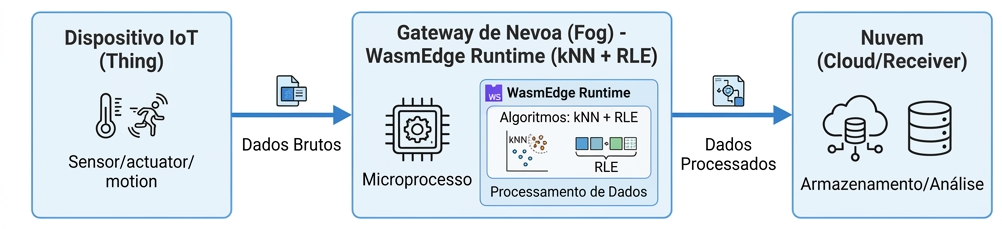
\includegraphics[width=12cm]{esquema_logico.png} 
\caption{Esquema lógico do pipeline: Sensor $\to$ Gateway LoRa $\to$ Processador (Névoa kNN+RLE) $\to$ Nuvem}
\label{fig:diagrama_blocos}
\fonte{O Autor (2026)}
\end{figure}

\begin{enumerate}
    \item \textbf{Dispositivo IoT (Thing/Simulador)}: Simula os nós sensores de campo. Ele lê dados brutos do ambiente (ou dados sintéticos KDE) e transmite via protocolo local para o gateway;
    \item \textbf{Gateway/Relay LoRa (LoRa)}: Atua como uma ponte de comunicação de rede, retransmitindo e roteando os pacotes HTTP/JSON entre o dispositivo IoT e o processador local na névoa;
    \item \textbf{Processador na Névoa (processador)}: Executa o runtime WasmEdge. Ele lê as variáveis físicas do buffer de entrada, normaliza os valores, classifica cada ponto pelo kNN ($k=3$) e codifica sequencialmente via RLE, retransmitindo a carga compactada;
    \item \textbf{Cloud Receiver (Nuvem)}: Recebe os dados processados e comprimidos do gateway/processador, realiza a descompressão e armazena-os na base persistente para visualização do usuário.
\end{enumerate}

\section{Componentes do Código e Implementação}

A arquitetura de software do projeto foi desenvolvida utilizando a linguagem Rust, visando alto desempenho, segurança de memória e facilidade de portabilidade. O ecossistema é composto por quatro programas principais localizados nos diretórios do projeto:

\subsection{Dispositivo IoT (simulador)}
O módulo \texttt{simulador} emula a coleta física dos sensores de temperatura e umidade da cultura de tomateiro. Ele é configurado para realizar requisições HTTP do tipo \texttt{POST} para o gateway de névoa, enviando a leitura no formato JSON.

\subsection{Gateway/Relay LoRa (LoRa)}
O módulo \texttt{LoRa} atua como o gateway/relay intermediário no pipeline de comunicação. Ele simula a interface de recepção e envio sem fio LPWAN de forma simplificada em nível de aplicação, atuando como um proxy retransmissor HTTP/JSON leve. Ele escuta conexões locais (porta padrão 8080) e aceita requisições do tipo \texttt{POST} nas rotas \texttt{/inserir} e \texttt{/receber}, retransmitindo os payloads para os respectivos componentes de processamento ou recepção.

\subsection{Processador na Névoa (processador)}
O módulo \texttt{processador} é o núcleo do ecossistema. Ele é compilado para WebAssembly (\texttt{wasm32-wasip1}) e executado sobre o runtime leve \texttt{WasmEdge}. Ele implementa:
\begin{itemize}
    \item A leitura e parsing das estruturas JSON correspondentes aos sensores;
    \item A base de dados de treinamento estática de 11 faixas de saúde do tomateiro;
    \item A normalização Min-Max e o algoritmo de busca e classificação de vizinhos $k$NN ($k=3$);
    \item O algoritmo de compressão Run-Length Encoding (RLE) temporal sobre a sequência de caracteres obtidos;
    \item Um gerador estocástico multivariado de dados sintéticos via KDE com ruído gaussiano (Box-Muller).
\end{itemize}

\subsection{Receptor na Nuvem (receiver)}
O módulo \texttt{receiver} atua como o servidor na nuvem que recebe as strings compactadas do processador, simula a descompressão dos dados de controle e realiza a escrita dos logs de recepção em um arquivo persistente (\texttt{monitoramento.txt}) para auditoria e exibição.

\subsection{Scripts de Validação e Análise em Python (gerador-de-dados)}
Além dos módulos em Rust executados no contínuo de IoT, o projeto conta com um conjunto de scripts utilitários desenvolvidos em Python (na pasta \texttt{gerador-de-dados/}) com o objetivo de realizar análises estatísticas de suporte e validação gráfica:
\begin{itemize}
    \item \texttt{gerar\_graficos\_artigo.py}: Este script é responsável pela geração das representações visuais equivalentes às Figuras 3 e 4 do artigo original de Ribeiro Junior et al. \cite{ribeiro2020nearest}. Ele carrega as séries temporais (tanto da base real quanto da base sintética gerada em Rust), classifica-as usando a mesma heurística normalizada do kNN, e gera as curvas de contorno de densidade conjunta e os correlogramas de dispersão de classes. Serve como ferramenta de validação visual e aderência topológica;
    \item \texttt{validar\_dados\_rust.py}: Atua como a suíte de testes estatísticos formais do gerador estocástico. Ele lê o arquivo original \texttt{entrada.csv} e o arquivo de dados sintéticos gerados pelo processador Rust (\texttt{dados\_sinteticos\_gerados\_rust.csv}), computa e imprime os p-valores do teste Kolmogorov-Smirnov (KS) de duas amostras para cada variável (temperatura e umidade), calcula os coeficientes de correlação linear de Pearson de ambas as distribuições para verificar a integridade da interdependência física das variáveis e gera gráficos comparativos de dispersão e histogramas.
\end{itemize}

\section{Fluxos de Execução do Processador}

O processador foi projetado com suporte a dois fluxos operacionais principais que atendem a cenários de rede distintos:

\subsection{Modo Normal (Online / Serviço HTTP)}
Neste modo, o processador atua como um servidor HTTP ativo escutando por requisições de sensores em tempo real. Ele expõe a rota \texttt{POST /inserir} para coletar leituras contínuas. Em segundo plano, uma rotina assíncrona (\textit{background thread}) rodando a cada 30 segundos agrupa os dados acumulados, executa a compactação RLE, envia os dados comprimidos para o receptor na nuvem (\texttt{POST /receber}) e limpa o buffer local para o próximo ciclo de monitoramento.

\subsection{Modo Lote (Offline / Batch Mode)}
Ativado pela passagem do argumento posicional \texttt{batch} na CLI, este fluxo destina-se ao processamento local de arquivos de sensores para campanhas offline e avaliações científicas de longa duração. Ele lê diretamente um arquivo CSV de entrada (ex.: \texttt{entrada.csv}), divide os dados em lotes com base em um tamanho de pacote configurável (via flag \texttt{--tamanho-pacote}), executa a classificação kNN e compressão RLE para cada lote, exporta estatísticas agregadas completas no formato JSON (\texttt{estatisticas\_compressao.json}) e finaliza a execução.

\subsection{Modo de Geração de Dados Sintéticos}
Quando a flag \texttt{--synthetic} (ou \texttt{--sintetico}) é especificada em conjunto com o modo \texttt{batch}, o processador executa a amostragem baseada na Estimativa de Densidade por Kernel (KDE) a partir do CSV de referência. Ele gera 40.000 registros sintéticos de temperatura e umidade aplicando ruído estocástico gaussiano via Box-Muller, salva a base sintética resultante em \texttt{dados\_sinteticos\_gerados\_rust.csv} e processa a cadeia simulada em lote sob as mesmas regras do Modo Lote offline.

\section{Outputs e Logs de Execução dos Componentes}

Para fins de validação operacional e documentação das saídas técnicas, os logs a seguir demonstram a inicialização e o tráfego de mensagens em tempo de execução de cada componente do ecossistema.

\subsection{Logs do Modo Normal (Online)}
O script de inicialização inicia o receptor de nuvem na porta 8082, seguido pelo processador do gateway na porta 8081 e pelo simulador de sensores. O log a seguir detalha a inicialização do processador na névoa:

\begin{lstlisting}[language=bash, caption={Log de inicialização do Processador na Névoa}]
==========================================
[INFO] Filtro rodando na porta 8081
[INFO] Ambiente: Fog
[INFO] Receiver alvo: http://localhost:8082/receber
[INFO] Ciclo de envio: 30 segundos
==========================================
Endpoints:
  POST /inserir     - Recebe dados dos sensores
  GET  /classificados - Lista dados classificados
  GET  /rle         - Aplica RLE e retorna compressao
  GET  /estatisticas - Estatisticas dos dados
  POST /reset       - Limpa todos os dados
==========================================
\end{lstlisting}

Durante a operação estável, conforme o simulador transmite dados de leitura, o processador imprime as operações de empacotamento e encaminhamento para a nuvem no final do timer de 30 segundos, conforme listado abaixo:

\begin{lstlisting}[language=bash, caption={Logs de recebimento e envio do gateway de névoa no Modo Normal}]
Requisicao recebida: POST /inserir
Requisicao recebida: POST /inserir
[SEND] Fog [Fog]: Enviando dados RLE para o Receiver...
[SUCCESS] Dados enviados com sucesso. Limpando armazenamento local...
[WAIT] Fog [Fog]: Sem dados para enviar neste ciclo.
\end{lstlisting}

O receptor de nuvem (\texttt{receiver}) exibe os logs de recepção e a taxa de redução dos dados empacotados pelo gateway, conforme o log a seguir:

\begin{lstlisting}[language=bash, caption={Log de recepção do Receiver na Nuvem}]
==========================================
[INFO] Receiver (Cloud) rodando na porta 8082
[INFO] Ambiente: Cloud
[INFO] Arquivo de log: monitoramento.txt
==========================================
[RECV] Receiver: Recebendo pacotes RLE...
[SAVE] Salvando string comprimida: 24O6P1G
[STATS] Reducao: 96.32%
\end{lstlisting}

\subsection{Logs do Modo Lote (Batch Offline)}
A execução offline do processamento em lote com a geração de dados sintéticos gera logs que detalham o carregamento da base, a amostragem probabilística e as taxas globais de redução calculadas. O output gerado pela execução do comando \texttt{wsl bash -l start\_all.sh 4 --synthetic} é listado abaixo:

\begin{lstlisting}[language=bash, caption={Log de execução do Processador no Modo Lote com Dados Sintéticos}]
==========================================
[START] Build concluido. Iniciando Modo: 4
==========================================
Configuracao 4: Processamento Offline em Lote (Batch Mode)
[INFO] Carregando dados base de entrada.csv...
[SUCCESS] 44023 registros carregados do CSV base.
[GEN] Gerando 40000 registros sinteticos usando KDE (bandwidth = 0.5)...
[SAVE] Salvando dados sinteticos gerados em 'dados_sinteticos_gerados_rust.csv'...
[SUCCESS] Arquivo 'dados_sinteticos_gerados_rust.csv' salvo com sucesso.
==========================================
[STATS] Relatorio de Processamento em Lote Gerado!
[FILE] Arquivo salvo em: estatisticas_compressao.json
[TOTAL] Total de registros processados: 40000
[SIZE] Tamanho original acumulado: 1856634 bytes
[kNN] Tamanho apos kNN: 40000 bytes (Reducao: 97.85%)
[RLE] Tamanho apos kNN+RLE: 69812 bytes (Reducao: 96.24%)
==========================================
\end{lstlisting}

Estes logs registram a execução exata dos experimentos de compactação utilizados para as discussões estatísticas e de engenharia de software presentes na seção de resultados.

% ==========================================================
\chapter{METODOLOGIA E CONFIGURAÇÃO EXPERIMENTAL}
\label{cap:metodologia}
% ==========================================================

\section{Ambiente de Execução Experimental}

Para garantir a reprodutibilidade de todas as avaliações de desempenho do ecossistema, os testes operacionais (envolvendo os quatro módulos Rust desenvolvidos) e as análises estatísticas em Python foram executados inteiramente em ambiente Linux. Especificamente, utilizou-se a distribuição Ubuntu instalada via subsistema Windows para Linux (WSL - \textit{Windows Subsystem for Linux}) executando sob um computador pessoal munido do sistema operacional Windows 11. As aplicações Rust compiladas para o target WebAssembly System Interface (\texttt{wasm32-wasip1}) foram executadas utilizando o runtime WasmEdge, o qual disponibiliza a sandbox e os recursos de rede adequados para emular a operação distribuída dos nós sensores e servidores locais.

\section{Detalhes de Implementação e Execução do Código}

A concretização prática do ecossistema distribuído envolveu a escrita de código em duas linguagens com propósitos distintos: Rust, para os componentes operacionais de tempo de execução no contínuo IoT, e Python, para os scripts de modelagem estatística, validação e plotagem de gráficos. Todo o código-fonte desenvolvido está hospedado publicamente no GitHub sob o repositório \href{https://github.com/v-cobof/pgc-rust}{\texttt{https://github.com/v-cobof/pgc-rust}}.

\subsection{Implementação dos Módulos em Rust}
Todos os quatro módulos Rust (\texttt{simulador}, \texttt{LoRa}, \texttt{processador} e \texttt{receiver}) compartilham de uma arquitetura modular voltada ao desempenho e segurança. As escolhas de crates (bibliotecas) foram orientadas para manter o footprint mínimo compatível com o target \texttt{wasm32-wasip1}:
\begin{itemize}
    \item \textbf{Crate \texttt{hyper}}: Utilizada nos módulos \texttt{processador} e \texttt{receiver} para estruturar os servidores HTTP. O \texttt{hyper} é uma biblioteca de rede de baixo nível e alto desempenho escrita em Rust, operando de forma assíncrona sobre o executor do \texttt{tokio};
    \item \textbf{Crate \texttt{reqwest}}: Utilizada nos componentes \texttt{simulador} e \texttt{LoRa} para realizar requisições HTTP do tipo cliente, disparando os payloads JSON na rede;
    \item \textbf{Crate \texttt{csv} e \texttt{serde}}: Empregadas para parsing e serialização de dados. O \texttt{csv} permite a leitura ultra-veloz de arquivos tabulares físicos (\texttt{entrada.csv}), enquanto o \texttt{serde} realiza a conversão bidirecional entre estruturas em memória e a representação textual JSON trafegada pela rede;
    \item \textbf{Crate \texttt{chrono}}: Utilizada para captura de tempos com alta precisão e escrita de logs em formato RFC3339 no \texttt{receiver}.
\end{itemize}

\subsection{Mapeamento de Diretórios na Sandbox WasmEdge}
Em tempo de execução, o runtime \texttt{WasmEdge} impõe isolamento de recursos (\textit{sandboxing}). Para permitir que os binários WASM acessem o sistema de arquivos local do gateway hospedeiro — necessário para ler a base de dados físicos \texttt{entrada.csv} no processador e persistir logs de texto (\texttt{monitoramento.txt}) ou relatórios JSON no receptor — é preciso habilitar explicitamente as capabilidades de E/S.

Isso foi realizado pela passagem da flag \texttt{--dir .} na linha de comando do WasmEdge, mapeando o diretório de execução atual no sistema de arquivos virtual da máquina virtual WASM. Sem esse mapeamento, qualquer tentativa de abertura de arquivos pelas APIs nativas do Rust (\texttt{std::fs::OpenOptions}) resultaria em falha de permissão de E/S (erro WASI de capabilidade negada).

\subsection{Estruturação dos Scripts Python}
Os scripts auxiliares em Python residem na pasta \texttt{gerador-de-dados/} e servem como o arcabouço de validação matemática e de plotagem de contornos:
\begin{itemize}
    \item \texttt{gerar\_dados\_sinteticos.py}: Utiliza a biblioteca \texttt{scikit-learn} para ajustar e amostrar do Kernel Density Estimator (\texttt{KernelDensity} com kernel gaussiano), além do \texttt{scipy.stats} para realizar o teste de normalidade de D'Agostino-Pearson e o teste KS;
    \item \texttt{validar\_dados\_rust.py} e \texttt{gerar\_graficos\_artigo.py}: Implementam a lógica comparativa de Pearson, teste KS de duas amostras e geram os gráficos científicos utilizando \texttt{matplotlib} e \texttt{seaborn} para as rodadas.
\end{itemize}

\section{O Dataset e o Modelo do Tomateiro}

O modelo agronômico do cultivo de tomateiro define faixas recomendadas de temperatura ($T$) e umidade ($H$). Neste projeto, o conjunto de treinamento da cultura de tomateiro está mapeado em 11 classes distintas de status, detalhadas na Tabela~\ref{tab:tomateiro}.

\begin{table}[H]
\centering
\caption{Tabela de treinamento e categorias da cultura de tomate}
\label{tab:tomateiro}
\begin{tabular}{cclcccc}
\toprule
\textbf{Categoria} & \textbf{Símbolo} & \textbf{Nome Agronômico} & \textbf{$T_{min}$} & \textbf{$T_{max}$} & \textbf{$H_{min}$} & \textbf{$H_{max}$} \\ \midrule
0 & D & Critical dry & 0,0 & 4,0 & 0,0 & 35,0 \\
1 & L & Lower fail & 0,0 & 11,0 & 40,0 & 65,0 \\
2 & M & Marginal & 12,0 & 28,0 & 40,0 & 55,0 \\
3 & U & Upper Fail & 29,0 & 47,0 & 40,0 & 55,0 \\
4 & C & Cold and Humid & 0,0 & 11,0 & 70,0 & 100,0 \\
5 & O & Lower optimal & 12,0 & 14,0 & 60,0 & 100,0 \\
6 & S & Optimal & 15,0 & 17,0 & 60,0 & 100,0 \\
7 & P & Upper Optimal & 18,0 & 27,0 & 60,0 & 100,0 \\
8 & E & Upper Marginal & 28,0 & 31,0 & 60,0 & 100,0 \\
9 & H & Upper Fail (high hum) & 32,0 & 35,0 & 60,0 & 100,0 \\
10 & K & Critical & 36,0 & 47,0 & 60,0 & 100,0 \\
\bottomrule
\end{tabular}
\fonte{Adaptado de Ribeiro Junior et al. \cite{ribeiro2020nearest}}
\end{table}

A base de dados físicos utilizada no experimento (\texttt{entrada.csv}) contém um histórico real de \textbf{44.023 leituras} contínuas coletadas por sensores físicos de temperatura e umidade relativa do ar. Os dados foram capturados com uma frequência de amostragem de 5 segundos, fornecendo leituras decimais precisas. A normalização Min-Max dos dados físicos utiliza os limites globais do sensor: para temperatura, $[0,0; 47,0]^\circ\text{C}$; para umidade, $[0,0; 100,0]\%$. O algoritmo $k$NN opera com $k=3$, calculando a distância Euclidiana com os centroides normalizados de cada classe da Tabela~\ref{tab:tomateiro}.

\section{Configuração dos Experimentos de Compressão}

Para analisar o desempenho do filtro de compressão e o seu impacto na latência e no volume de rede, avaliamos o processo sob 5 tamanhos de lote de transmissão (tamanho do pacote acumulado no gateway antes da aplicação do codificador RLE):
\begin{itemize}
    \item \textbf{Lote 6} (janela temporal de 30 segundos de dados físicos): Simula uma transmissão de alta frequência e baixa latência (tempo real de monitoramento via redes LPWAN/LoRa);
    \item \textbf{Lote 60} (janela temporal de 5 minutos): Representa telemetria típica de sensores agrícolas em ciclos regulares;
    \item \textbf{Lote 720} (janela temporal de 1 hora): Mapeia relatórios agronômicos de hora em hora para análise de tendências climáticas;
    \item \textbf{Lote 4.320} (janela temporal de 6 horas): Agrupa dados por turnos de trabalho (por exemplo, período da madrugada vs. manhã);
    \item \textbf{Lote 20.000} (janela temporal de aproximadamente 14 horas de dados contínuos): Representa uma grande carga de dump de dados diários offline.
\end{itemize}

O experimento de compressão em lote foi executado 3 vezes independentes. Em cada rodada, gerou-se uma nova base de dados sintéticos via KDE com 40.000 leituras, de modo a garantir a análise de robustez estatística frente à variabilidade estocástica do gerador Rust.

\section{Planilha de Métricas de Validação}

A validação científica da geração de dados estocásticos utilizou três métricas fundamentais:
\begin{enumerate}
    \item \textbf{Teste KS de Duas Amostras}: Aplica-se às séries de temperatura e umidade separadamente. O p-valor limite de rejeição da hipótese nula de igualdade é $\alpha = 0,05$. Se $p > 0,05$, considera-se que o gerador Rust reproduz fielmente a distribuição de probabilidade da base física;
    \item \textbf{Coeficiente de Correlação de Pearson ($r$)}: Calcula-se o coeficiente linear entre temperatura e umidade para a base real ($r_{orig}$) e para a base sintética ($r_{rust}$); a diferença absoluta $|r_{orig} - r_{rust}|$ deve ser inferior a $0,01$;
    \item \textbf{Comparação de Curvas de Contorno e Correlogramas}: Avaliação visual das densidades bidimensionais e da dispersão espacial das classes kNN nas sub-rodadas (Round 1 e Round 2) para verificar a aderência topológica dos dados simulados.
\end{enumerate}

% ==========================================================
\chapter{RESULTADOS E DISCUSSÃO}
\label{cap:resultados}
% ==========================================================

\section{Validação Estatística dos Dados Sintéticos}

Os testes estatísticos provaram que o gerador estocástico baseado na estimativa KDE multivariada e implementado em Rust com a transformada de Box-Muller apresenta altíssima fidelidade científica na reprodução do comportamento do sensor físico real.

O teste de Kolmogorov-Smirnov (KS) \cite{massey1951ks} de duas amostras comparou 44.023 leituras reais contra 40.000 leituras sintéticas. O resultado para a temperatura apresentou estatística $D = 0,0080$ com p-valor de $0,1385$. Para a umidade, a estatística obtida foi $D = 0,0040$ com p-valor de $0,8974$. Sendo ambos os p-valores amplamente superiores a $0,05$, aceita-se a hipótese nula $H_0$ de que ambas as amostras provêm da mesma distribuição populacional contínua.

A correlação física inversa entre temperatura e umidade foi preservada com precisão. O coeficiente de Pearson \cite{pearson1895} dos dados originais foi calculado em $r_{orig} = -0,8837$, enquanto a base sintética apresentou $r_{rust} = -0,8804$. A diferença absoluta obtida foi de apenas $0,0033$ (desvio de $0,37\%$), demonstrando que o gerador multivariado reproduz com exatidão a interdependência física das variáveis.

\section{Análise Visual das Curvas de Densidade e Distribuição}

A comparação visual das densidades de probabilidade e da classificação espacial revela um comportamento estatístico fundamental sobre o processo de emulação. A Figura~\ref{fig:densidade_original_sintetico} exibe os gráficos de contorno de densidade (equivalentes à Figura 3 do artigo de base) comparando as rodadas reais de dados com as amostras sintéticas correspondentes.

\begin{figure}[H]
\centering
\begin{subfigure}[b]{0.49\textwidth}
    \centering
    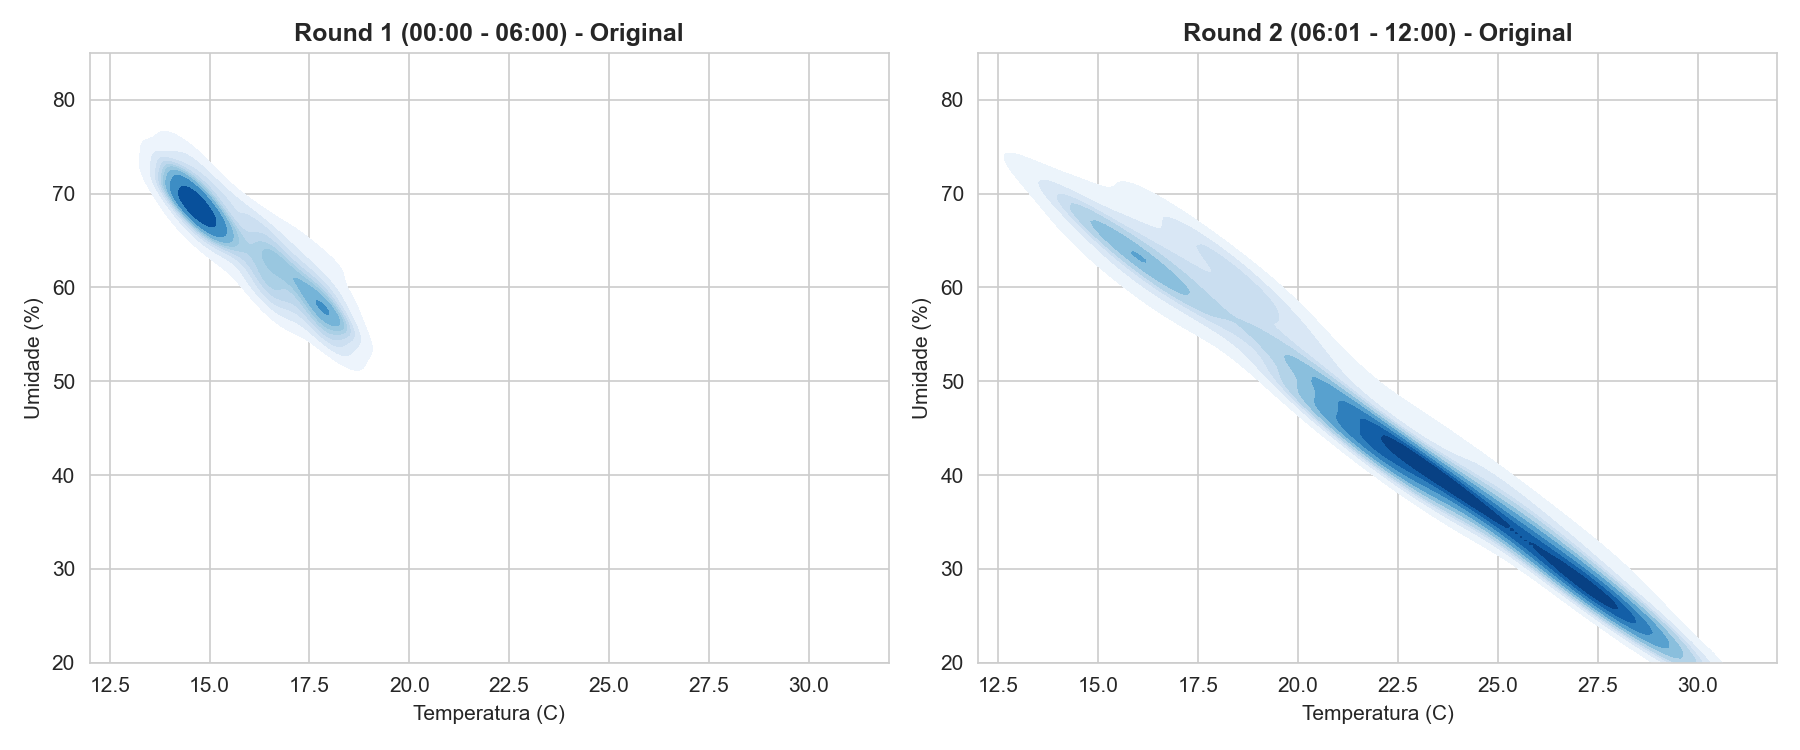
\includegraphics[width=\textwidth]{analise-experimentos/densidade_artigo_original.png}
    \caption{Dados Reais (Round 1 e Round 2)}
\end{subfigure}
\hfill
\begin{subfigure}[b]{0.49\textwidth}
    \centering
    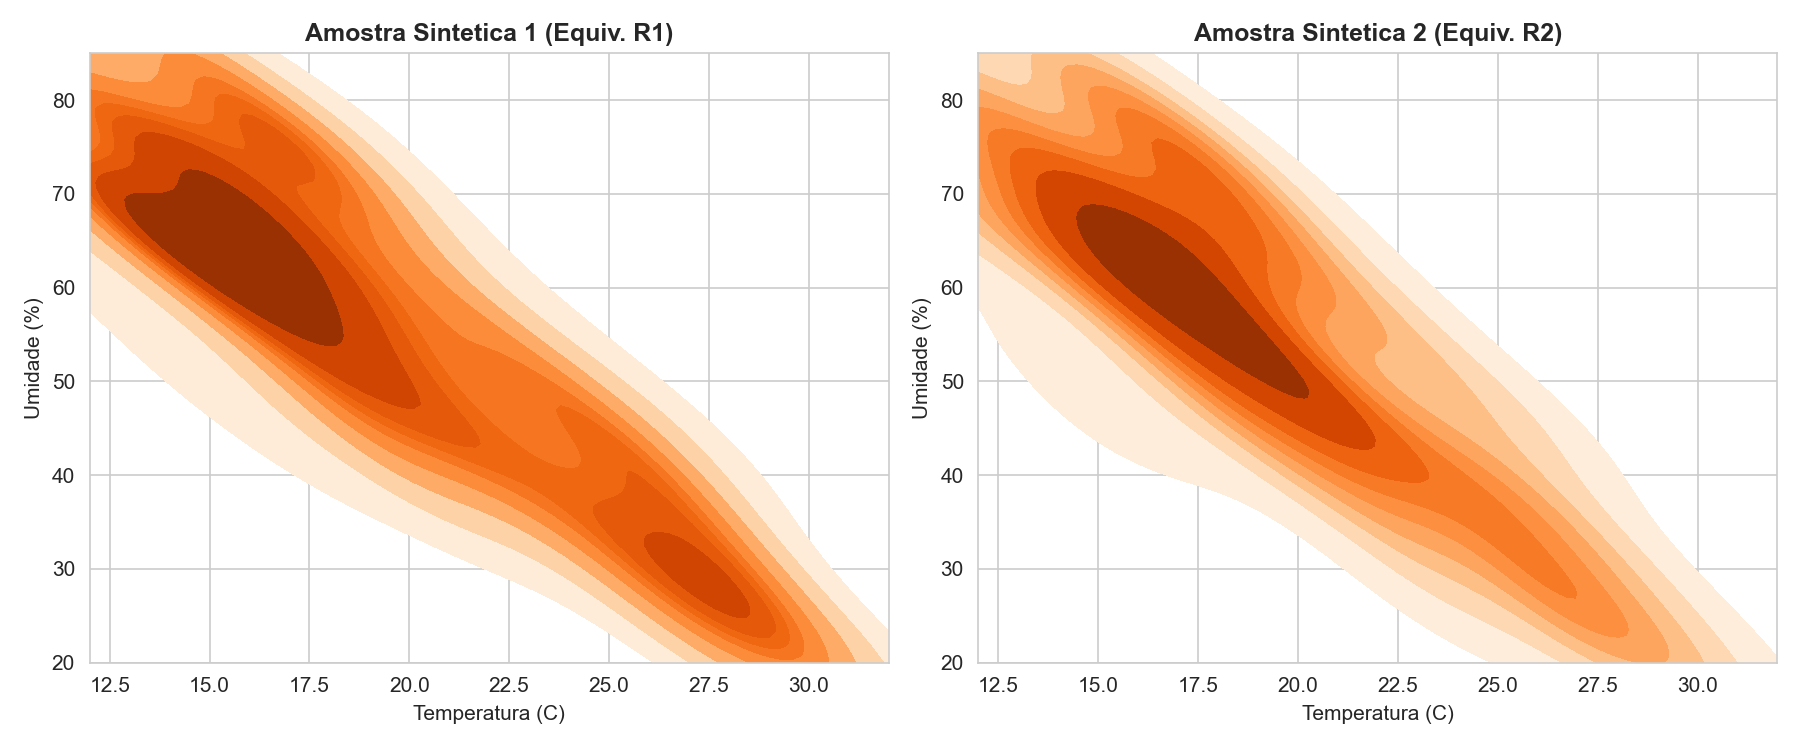
\includegraphics[width=\textwidth]{analise-experimentos/densidade_artigo_sintetico.png}
    \caption{Dados Sintéticos KDE}
\end{subfigure}
\caption{Curvas de contorno de densidade de probabilidade bidimensional}
\label{fig:densidade_original_sintetico}
\fonte{O Autor (2026)}
\end{figure}

Percebe-se que as curvas de contorno dos dados originais (Figura~\ref{fig:densidade_original_sintetico}a) exibem padrões térmicos e de umidade bem delimitados para cada rodada: o Round 1 (período da madrugada) apresenta-se como um cluster concentrado em baixas temperaturas e alta umidade, enquanto o Round 2 (período da manhã) estende-se em uma longa faixa diagonal conforme a temperatura se eleva. Contudo, nas curvas dos dados sintéticos (Figura~\ref{fig:densidade_original_sintetico}b), tanto a Amostra Sintética 1 quanto a Amostra Sintética 2 apresentam comportamentos quase idênticos, ocupando toda a amplitude diagonal da base completa. 

Essa diferença decorre do fato de que o gerador estocástico baseado em KDE é um modelo probabilístico estático e \textit{i.i.d.} (independente e identicamente distribuído). Ele estima a função de densidade conjunta global a partir de todo o conjunto de dados da base física e gera novos pontos por amostragem espacial, sem modelar a correlação temporal ou a ordenação cronológica da série original. Como resultado, ao dividir a base sintética em duas metades ordenadas para representar as duas rodadas temporais, ambas as metades contêm amostras aleatórias que refletem a densidade global conjunta, e não as restrições térmicas locais de cada período.

Os correlogramas detalhados com a coloração dos pontos pelas classes classificadas pelo algoritmo $k$NN ($k=3$), com as curvas de densidade marginais integradas nos eixos (equivalentes à Figura 4 do artigo), são apresentados para as sub-rodadas nas Figuras~\ref{fig:correlograma_r1} e \ref{fig:correlograma_r2}.

\begin{figure}[H]
\centering
\begin{subfigure}[b]{0.49\textwidth}
    \centering
    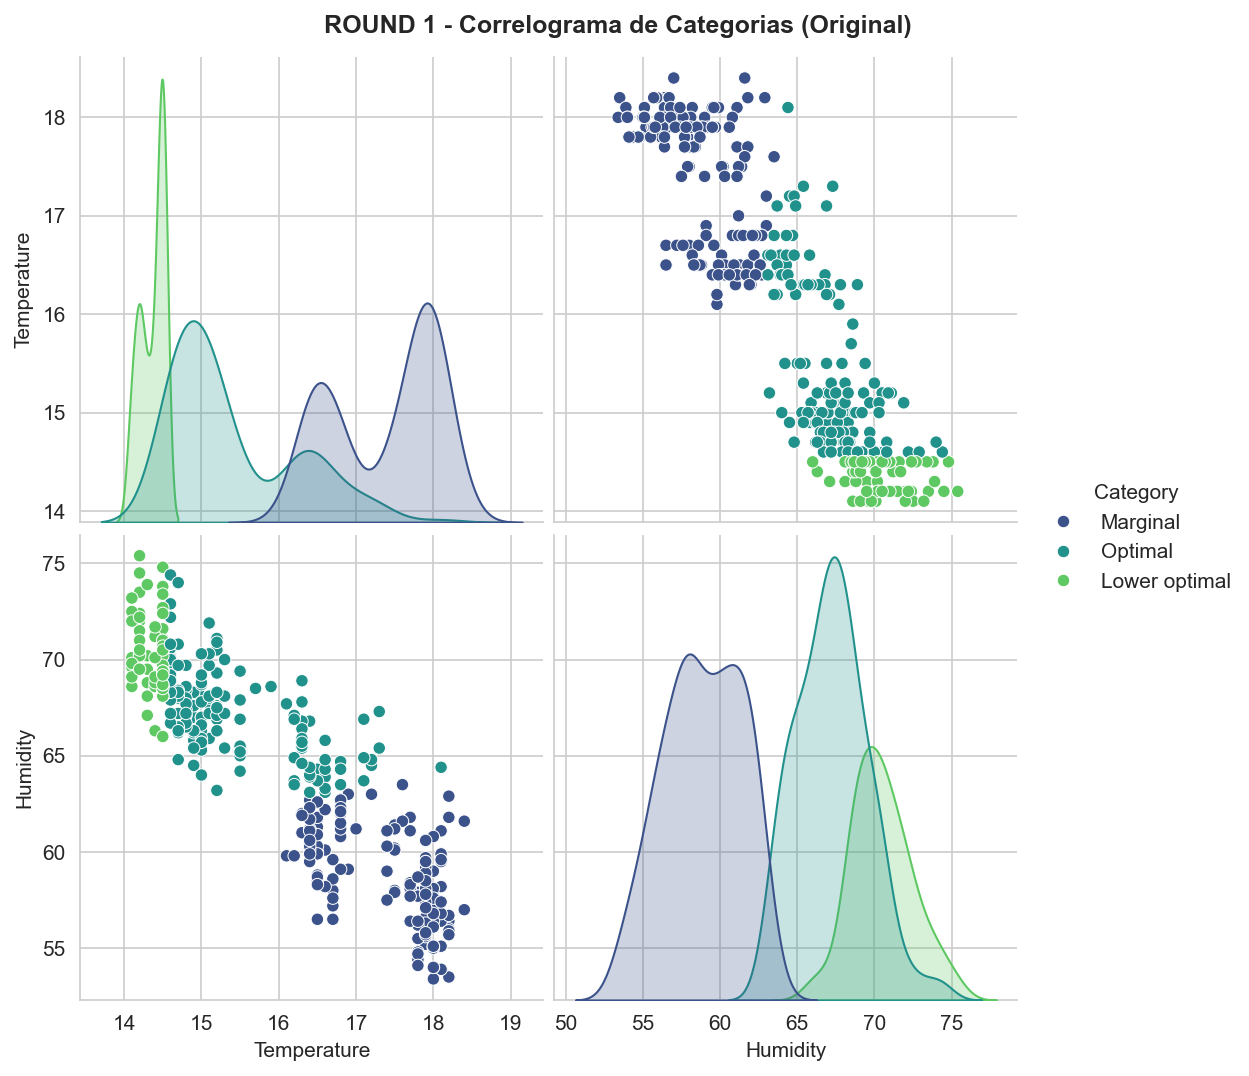
\includegraphics[width=\textwidth]{analise-experimentos/correlograma_r1_original.png}
    \caption{Round 1 - Original}
\end{subfigure}
\hfill
\begin{subfigure}[b]{0.49\textwidth}
    \centering
    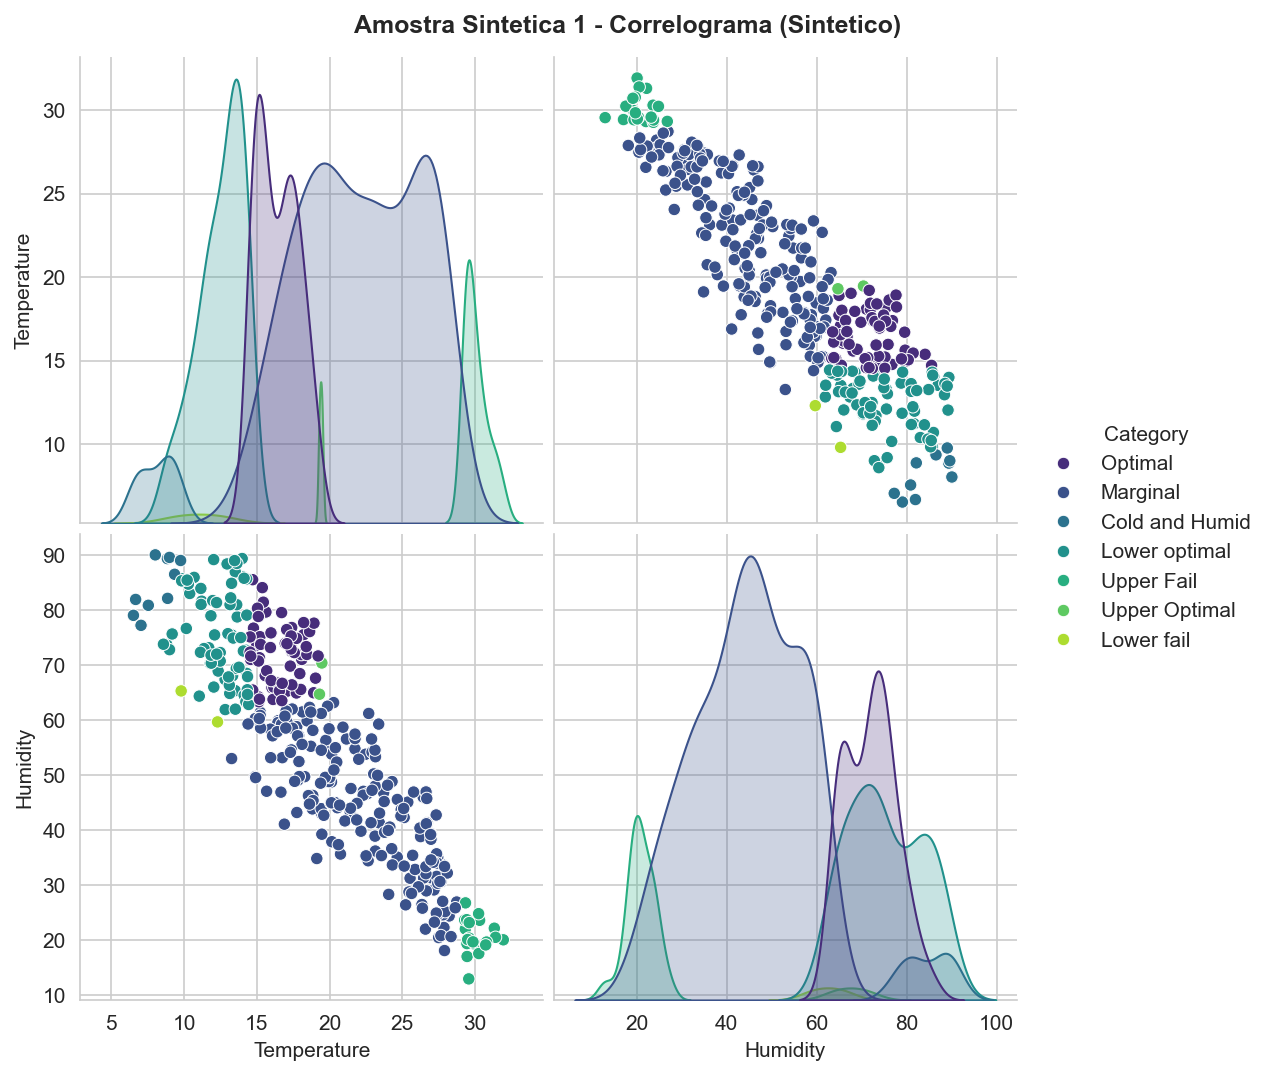
\includegraphics[width=\textwidth]{analise-experimentos/correlograma_r1_sintetico.png}
    \caption{Round 1 - Sintético}
\end{subfigure}
\caption{Correlogramas de Temperatura vs Umidade classificados por kNN (Round 1)}
\label{fig:correlograma_r1}
\fonte{O Autor (2026)}
\end{figure}

\begin{figure}[H]
\centering
\begin{subfigure}[b]{0.49\textwidth}
    \centering
    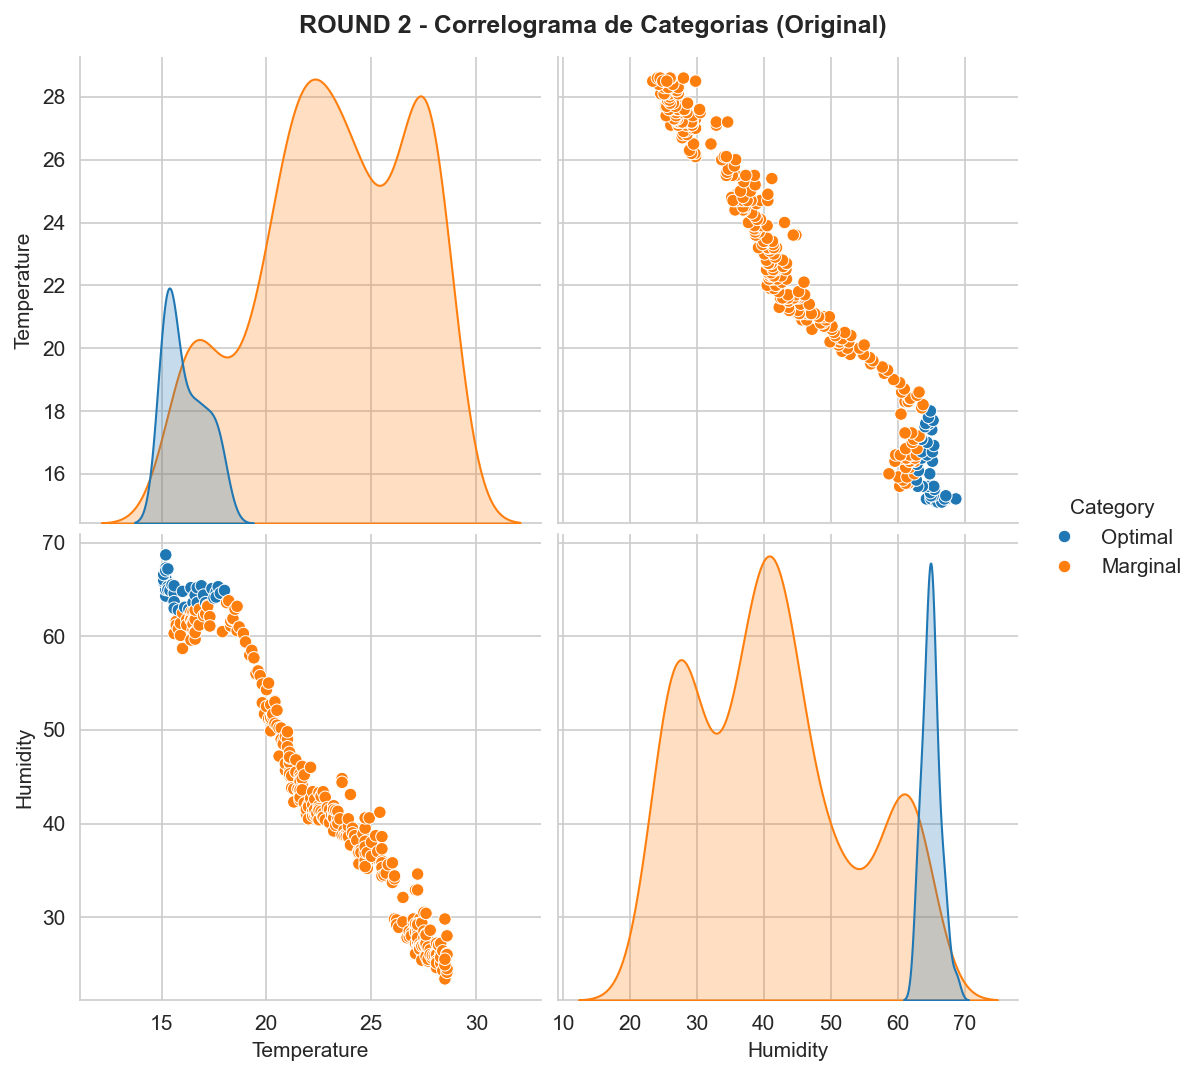
\includegraphics[width=\textwidth]{analise-experimentos/correlograma_r2_original.png}
    \caption{Round 2 - Original}
\end{subfigure}
\hfill
\begin{subfigure}[b]{0.49\textwidth}
    \centering
    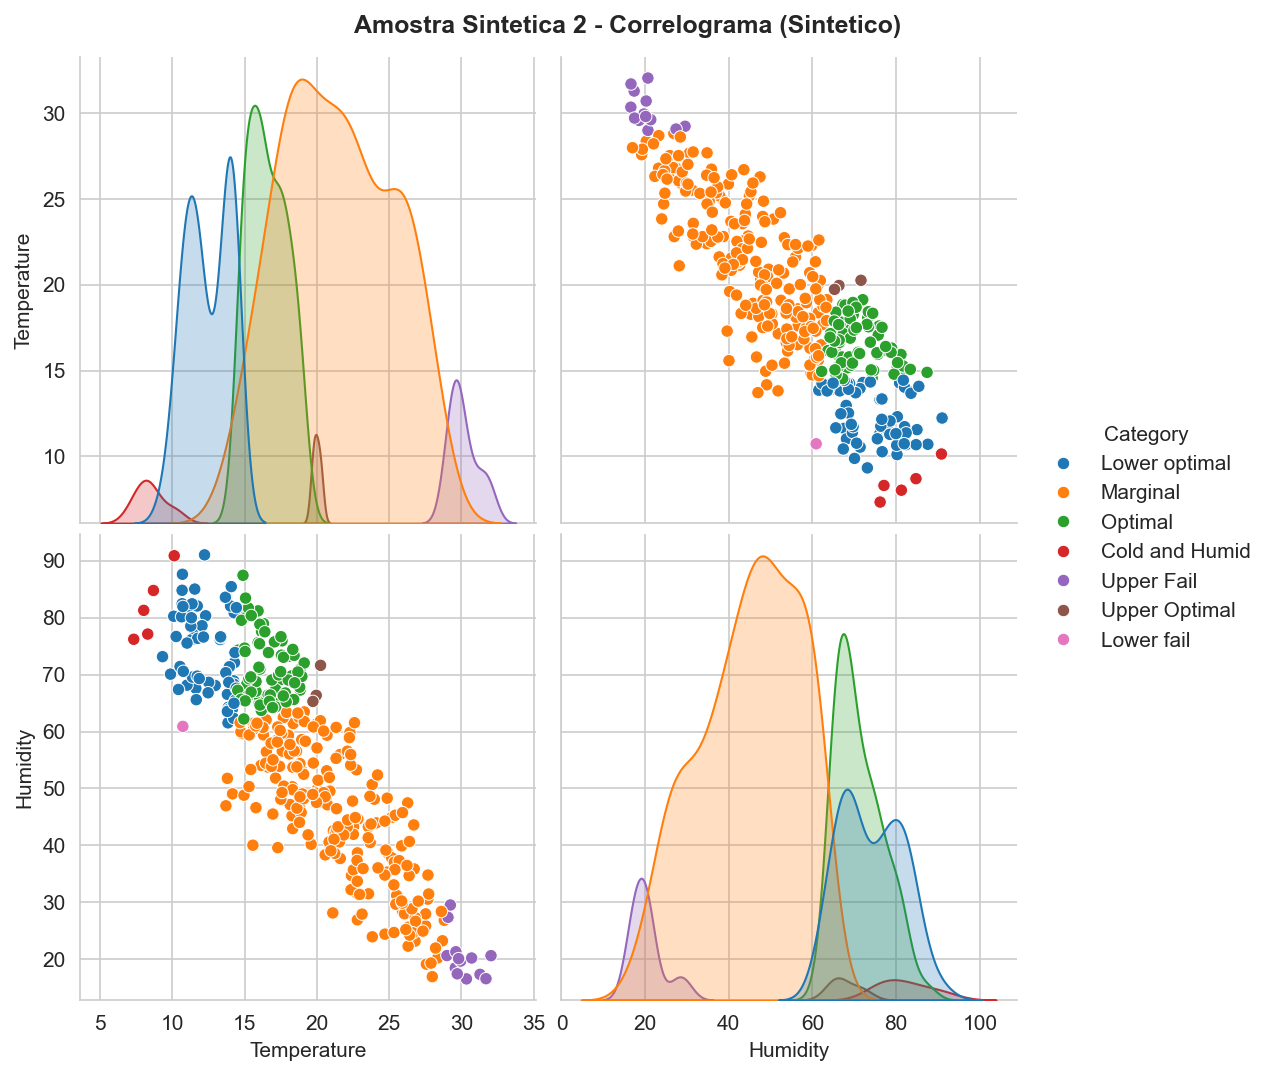
\includegraphics[width=\textwidth]{analise-experimentos/correlograma_r2_sintetico.png}
    \caption{Round 2 - Sintético}
\end{subfigure}
\caption{Correlogramas de Temperatura vs Umidade classificados por kNN (Round 2)}
\label{fig:correlograma_r2}
\fonte{O Autor (2026)}
\end{figure}

Os correlogramas evidenciam a mesma característica estrutural. Enquanto os dados originais do Round 1 (Figura~\ref{fig:correlograma_r1}a) concentram-se em temperaturas de 14 a 19${}^\circ\text{C}$ e classificam os pontos em apenas 3 categorias (\textit{Marginal}, \textit{Optimal} e \textit{Lower optimal}), a versão sintética correspondente (Figura~\ref{fig:correlograma_r1}b) exibe pontos dispersos ao longo de todo o espectro do dataset global (de 5 a 30${}^\circ\text{C}$), ativando classes adicionais como \textit{Upper Fail} e \textit{Cold and Humid}. As distribuições marginais de temperatura e umidade ao longo dos eixos confirmam que as metades sintéticas simulam a densidade global conjunta.

Finalmente, a Figura~\ref{fig:densidade_global} apresenta a comparação global de contorno bidimensional para a base completa de dados reais e sintéticos.

\begin{figure}[H]
\centering
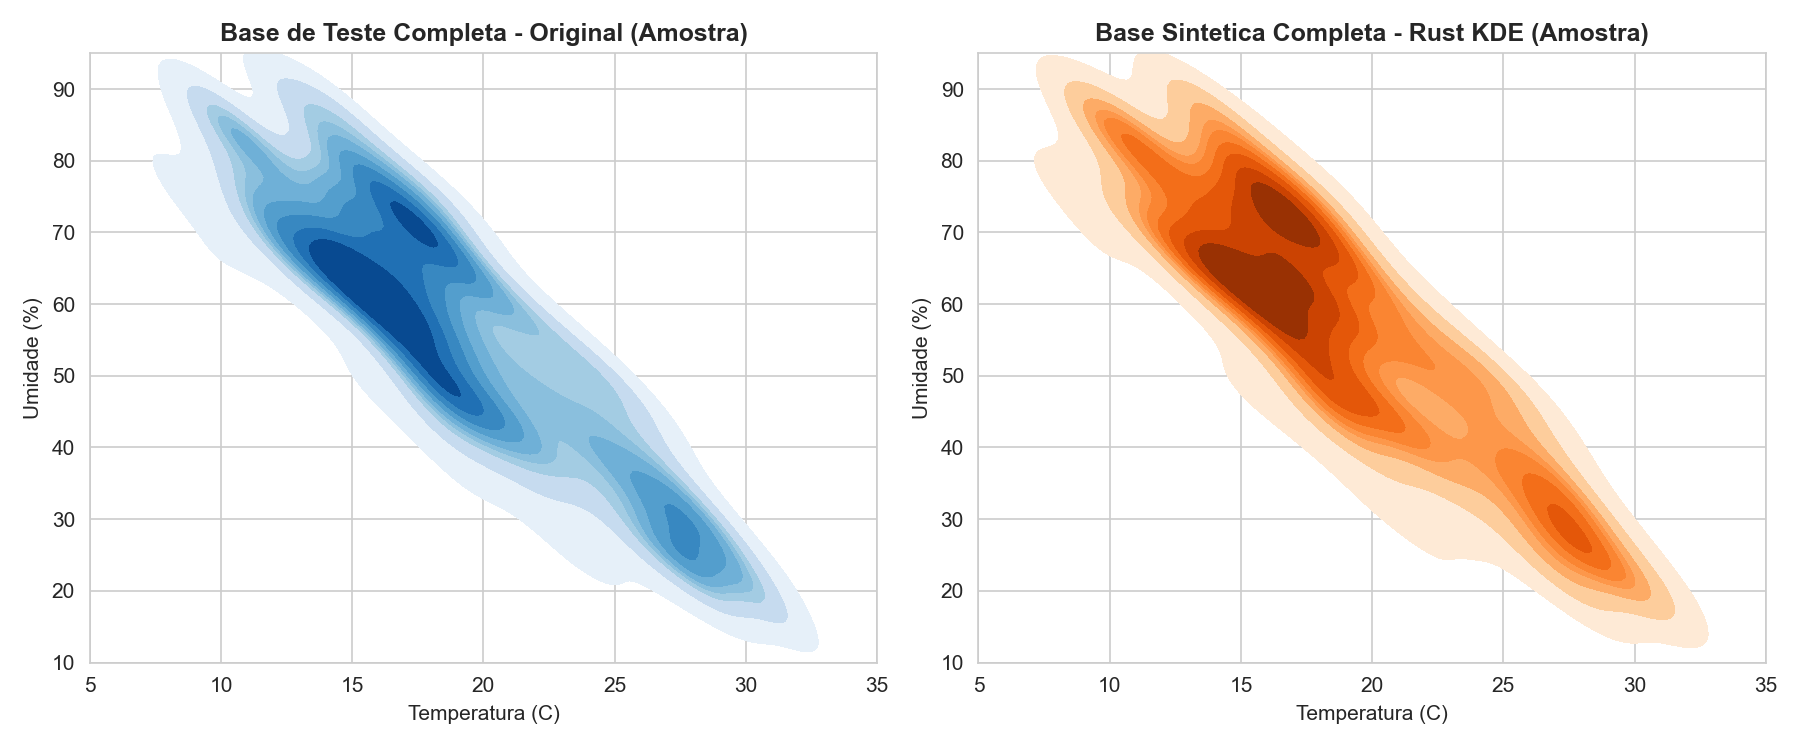
\includegraphics[width=11cm]{analise-experimentos/densidade_global_comparacao.png}
\caption{Comparação de Densidade Bidimensional Completa (Original vs Sintético)}
\label{fig:densidade_global}
\fonte{O Autor (2026)}
\end{figure}

A sobreposição visual na Figura~\ref{fig:densidade_global} confirma que, sob uma perspectiva de distribuição acumulada global, o gerador KDE em Rust recupera a estrutura estocástica latente com de fato altíssima fidelidade, apresentando contornos e centros de adensamento muito próximos aos da base física real. Entretanto, a perda da ordenação temporal inerente à amostragem \textit{i.i.d.} do KDE introduz uma flutuação de alta frequência nas séries sintéticas. Em dados reais, a temperatura e a umidade mudam lentamente no tempo (baixa frequência), gerando longas sequências contínuas da mesma classe agronômica. Na série sintética, a flutuação \textit{i.i.d.} faz com que a classe classificada pelo kNN oscile rapidamente entre pontos adjacentes. Esse ruído artificial de alta frequência encurta o comprimento médio das corridas contíguas, o que explica por que o codificador RLE apresenta menor ganho de compressão nos dados simulados do que nos dados reais sequenciais, servindo como uma importante diretriz empírica para projetistas de simuladores de sensores IoT.

\section{Resultados da Compressão de Dados nos Experimentos}

Para caracterizar o impacto do empacotamento na compressão, realizou-se a segmentação da base de dados simulada de 40.000 registros em 5 cenários de lotes distintos. A Tabela~\ref{tab:simulacao_lote_detalhe} apresenta a modelagem e a partição temporal do experimento para a primeira bateria de testes (Experimento 1).

\begin{table}[H]
\centering
\caption{Detalhamento da partição dos dados em lotes no Experimento 1}
\label{tab:simulacao_lote_detalhe}
\resizebox{\textwidth}{!}{%
\begin{tabular}{ccrccc}
\toprule
\textbf{Tamanho do Lote} & \textbf{Escopo Temporal} & \textbf{Qtd. de Lotes} & \textbf{Original Acumulado (B)} & \textbf{kNN Acumulado (B)} & \textbf{RLE Acumulado (B)} \\ \midrule
6 & 30 segundos (Micro) & 6.667 & 1.856.634 & 40.000 & 70.218 \\
60 & 5 minutos & 667 & 1.850.634 & 40.000 & 68.288 \\
720 & 1 hora & 56 & 1.850.023 & 40.000 & 68.062 \\
4.320 & 6 horas & 10 & 1.849.977 & 40.000 & 67.962 \\
20.000 & ~14 horas (Metade) & 2 & 1.849.969 & 40.000 & 68.104 \\
\bottomrule
\end{tabular}%
}
\fonte{O Autor (2026)}
\end{table}

A partir do detalhamento de partição, dois fenômenos de engenharia de software e análise de dados podem ser formalizados:

\subsection{Custo de Serialização JSON e o Overhead de Colchetes}
Observa-se na Tabela~\ref{tab:simulacao_lote_detalhe} que o tamanho acumulado dos dados originais (em formato JSON bruto) diminui à medida que o tamanho do lote aumenta, passando de 1.856.634 bytes para 1.849.969 bytes (uma redução líquida de 6.665 bytes). Isso é explicado pelo custo de sintaxe da estrutura de matriz JSON (\texttt{[...]}). Cada lote processado adiciona dois caracteres sintáticos (um colchete de abertura e um de fechamento) à string serializada.
\begin{itemize}
    \item Para lote de tamanho 6, a divisão resulta em 6.667 lotes independentes, introduzindo um overhead de aproximadamente 13.334 bytes apenas em colchetes delimitadores.
    \item Para lote de tamanho 20.000, o overhead sintático cai para apenas 4 bytes no total (referente aos colchetes dos 2 lotes gerados).
\end{itemize}

\subsection{Efeito de Borda e o Lote Ideal}
O ponto de maior compressão para a técnica combinada kNN+RLE ocorreu de forma consistente no tamanho de \textbf{4.320 registros (6 horas)}, resultando em um payload de \textbf{67.962 bytes}. Isso decorre da redução do ``efeito de borda'': à medida que o tamanho do pacote aumenta, a probabilidade de uma corrida longa de categorias ser artificialmente interrompida na fronteira de divisão do lote diminui. Isso permite ao RLE formar sequências mais compactas.
Contudo, para lotes ainda maiores, como o de \textbf{20.000 registros}, o ganho é ligeiramente degradado (subindo para 68.104 bytes). Esse fenômeno decorre da representação numérica decimal das frequências no RLE. Frequências muito longas demandam mais caracteres decimais (exemplo: representar uma contagem de $12.345$ repetições da classe \texttt{Optimal} consome 6 bytes, \texttt{12345O}, enquanto contagens menores na faixa de dezenas ou centenas consomem de 2 a 3 bytes). O custo extra dos dígitos numéricos adicionais anula as vantagens marginais obtidas na eliminação das quebras de borda.

\subsection{Consistência entre Execuções Independentes}
Para validar a estabilidade estatística do gerador, os experimentos de compressão foram repetidos em três baterias completas com novos dados estocásticos gerados via KDE. A Tabela~\ref{tab:tamanhos_comprimidos} apresenta o tamanho final do payload em bytes após a codificação kNN+RLE para cada bateria.

\begin{table}[H]
\centering
\caption{Tamanhos finais após compactação kNN+RLE (Bytes)}
\label{tab:tamanhos_comprimidos}
\resizebox{\textwidth}{!}{%
\begin{tabular}{cccccc}
\toprule
\textbf{Tamanho do Lote} & \textbf{Experimento 1} & \textbf{Experimento 2} & \textbf{Experimento 3} & \textbf{Desvio Máx.} & \textbf{Var. \% Máx.} \\ \midrule
6 & 70.218 & 70.142 & 70.038 & 180 B & $0,25\%$ \\
60 & 68.288 & 67.982 & 68.166 & 306 B & $0,44\%$ \\
720 & 68.062 & 68.072 & 67.932 & 140 B & $0,20\%$ \\
4.320 & 67.962 & 68.194 & 68.022 & 232 B & $0,34\%$ \\
20.000 & 68.104 & 68.082 & 68.100 & 22 B & $0,03\%$ \\
\bottomrule
\end{tabular}%
}
\fonte{O Autor (2026)}
\end{table}

A variação máxima observada entre as execuções independentes foi extremamente reduzida (abaixo de $0,44\%$). Como kNN e RLE são determinísticos, essa flutuação residual decorre unicamente da semente aleatória do gerador estocástico KDE que altera ligeiramente as coordenadas dos pontos de dados simulados nas fronteiras de decisão das classes do tomateiro, alterando pontualmente os padrões de alternância de classes. Isso comprova a elevada estabilidade estatística e reprodutibilidade do gerador.

A Tabela~\ref{tab:taxas_reducao} resume as taxas de compressão percentual obtidas para as três baterias de teste em relação à representação original serializada em JSON.

\begin{table}[H]
\centering
\caption{Taxas de redução acumuladas (kNN+RLE) em relação ao JSON original (\%)}
\label{tab:taxas_reducao}
\resizebox{\textwidth}{!}{%
\begin{tabular}{ccccc}
\toprule
\textbf{Tamanho do Lote} & \textbf{Experimento 1 (\%)} & \textbf{Experimento 2 (\%)} & \textbf{Experimento 3 (\%)} & \textbf{Variação Máx. (\%)} \\ \midrule
6 & $96,22\%$ & $96,22\%$ & $96,23\%$ & $0,01\%$ \\
60 & $96,31\%$ & $96,33\%$ & $96,32\%$ & $0,02\%$ \\
720 & $96,32\%$ & $96,32\%$ & $96,33\%$ & $0,01\%$ \\
4.320 & $96,33\%$ & $96,31\%$ & $96,32\%$ & $0,02\%$ \\
20.000 & $96,32\%$ & $96,32\%$ & $96,32\%$ & $0,00\%$ \\
\bottomrule
\end{tabular}%
}
\fonte{O Autor (2026)}
\end{table}

Percebe-se que, independente do tamanho de lote utilizado e das flutuações amostrais, a taxa de redução global de dados transmitidos fica estavelmente posicionada acima de $96,2\%$.


\section{Comparação kNN Puro vs kNN+RLE}

Uma das contribuições mais relevantes deste estudo emerge da comparação direta entre o uso de apenas a classificação kNN (kNN Puro) e a combinação de classificação com codificação de corrida (kNN+RLE). A Tabela~\ref{tab:pure_vs_rle} traz a comparação média das taxas de redução.

\begin{table}[H]
\centering
\caption{Comparação de redução: kNN Puro vs kNN+RLE}
\label{tab:pure_vs_rle}
\resizebox{\textwidth}{!}{%
\begin{tabular}{cccl}
\toprule
\textbf{Tamanho do Lote} & \textbf{Redução kNN Puro (\%)} & \textbf{Redução kNN+RLE (\%)} & \textbf{Melhor Opção} \\ \midrule
6 (30 s) & $97,85\%$ (40 KB) & $96,22\%$ (70 KB) & \textbf{kNN Puro} ($+1,63\%$) \\
60 (5 min) & $97,84\%$ (40 KB) & $96,32\%$ (68 KB) & \textbf{kNN Puro} ($+1,52\%$) \\
720 (1 h) & $97,84\%$ (40 KB) & $96,31\%$ (68 KB) & \textbf{kNN Puro} ($+1,53\%$) \\
4.320 (6 h) & $97,84\%$ (40 KB) & $96,32\%$ (68 KB) & \textbf{kNN Puro} ($+1,52\%$) \\
20.000 (14 h) & $97,84\%$ (40 KB) & $96,32\%$ (68 KB) & \textbf{kNN Puro} ($+1,52\%$) \\
\bottomrule
\end{tabular}%
}
\fonte{O Autor (2026)}
\end{table}

Os dados revelam uma constatação contra-intuitiva: \textbf{o kNN Puro comprime mais e gera payloads menores do que o kNN+RLE em todas as configurações}. O kNN Puro reduziu o arquivo final para estáveis 40 KB, enquanto o RLE resultou em arquivos entre 68 KB e 70 KB.

\subsection{Discussão sobre a Ineficiência do RLE}

Esse comportamento deve-se a dois fatores principais decorrentes do alfabeto de símbolos curto do classificador $k$NN:

\begin{enumerate}
    \item \textbf{Fenômeno de Expansão de Símbolo Único}:
    O kNN converte cada par de leituras físicas em uma string de um caractere (por exemplo, \texttt{O} para \textit{Optimal}). Portanto, 40.000 leituras correspondem a 40.000 caracteres de texto puro, ocupando exatamente 40.000 bytes.
    Quando o RLE atua, ele agrupa caracteres repetidos na estrutura \texttt{<frequência><categoria>} (ex: \texttt{3O}). Para leituras com baixa repetição consecutiva (comprimento de corrida $C = 1$), o RLE codifica a ocorrência como \texttt{1O} (ocupando \textbf{2 bytes}, o que representa uma expansão de $100\%$ do tamanho original de $1$ byte).
    
    \item \textbf{Oscilação Natural do Sensor Físico (Ruído de Fronteira)}:
    Como temperatura e umidade flutuam continuamente sob efeito de ruído físico na bacia de captação dos sensores, os dados próximos aos limites de decisão do classificador $k$NN oscilam constantemente de classe (por exemplo, alternando entre \texttt{O}, \texttt{P} e \texttt{S} a cada minuto). Essas alternâncias de alta frequência rompem a homogeneidade das corridas contíguas. 
    A grande quantidade de corridas de comprimento unitário ou muito curtas geradas pela variabilidade dos dados causa uma expansão de volume que anula a economia de espaço proporcionada pelas raras corridas longas, resultando em um payload total acumulado de 68 KB a 70 KB para o RLE contra os 40 KB estáveis do kNN Puro.
\end{enumerate}

Essa análise revela que a compactação RLE é inadequada se a codificação do kNN já foi previamente otimizada para 1 caractere de comprimento. O RLE só apresentaria vantagem se o kNN puro exportasse rótulos textuais completos (como \texttt{"Optimal"} e \texttt{"Upper Marginal"}), caso em que o custo de strings de 7 a 15 bytes justificaria o overhead de adicionar contadores.

% ==========================================================
\chapter{CONCLUSÃO}
\label{cap:conclusao}
% ==========================================================

Este trabalho apresentou uma abordagem robusta e eficiente para a computação em névoa aplicada à IoT agrícola. A migração dos algoritmos de classificação kNN e compressão de dados para Rust compilado em WebAssembly demonstrou a viabilidade de implantar soluções analíticas de alta segurança e portabilidade em gateways de borda reais com baixíssimo consumo de recursos computacionais.

O simulador estocástico desenvolvido em Rust/WASM, fundamentado na Estimativa de Densidade por Kernel (KDE) e na Transformada de Box-Muller, comprovou ser uma ferramenta científica valiosa para modelar e gerar de forma altamente precisa dados sintéticos de sensores locais. Os testes Kolmogorov-Smirnov e a correlação de Pearson atestaram a excelente representatividade física dos dados simulados.

Os experimentos de compressão revelaram a ineficiência prática da combinação do $k$NN com o RLE em relação ao $k$NN puro quando o formato do status agronômico já é otimizado para caracteres únicos de 1 byte. Esse resultado contraria suposições teóricas comuns de projetos de transmissão IoT e serve como uma diretriz empírica crucial para projetistas de sistemas de monitoramento agrícola.

Como trabalhos futuros, propõe-se a validação em campo utilizando gateways LoRaWAN físicos baseados em arquiteturas ARM de baixo custo executando WasmEdge. Sugere-se também a investigação de algoritmos de classificação adaptativos que ajustem dinamicamente o valor de $k$ com base no nível de bateria disponível nos nós sensores, e a aplicação de classificadores robustos a ruídos de fronteira de modo a minimizar as oscilações de classificação que degradam a eficiência da codificação temporal.

% ----------------------------------------------------------
% REFERÊNCIAS
% ----------------------------------------------------------
\bibliography{references}

% --- Apêndices ---
\begin{apendicesenv}

\chapter{ESTRUTURA DO PROJETO DE SENSORES E NÉVOA}

A estrutura de diretórios do ecossistema PGC-Rust está organizada da seguinte forma:

\begin{lstlisting}[language=bash, caption={Estrutura de diretórios do PGC-Rust}]
pgc-rust/
|-- processador/             # Modulo da Nevoa (WASM)
|   |-- Cargo.toml
|   |-- src/
|   |   |-- main.rs          # Algoritmo kNN, RLE e Gerador KDE
|-- simulador/               # Componente do dispositivo IoT (Thing)
|   |-- Cargo.toml
|   |-- src/
|   |   |-- main.rs
|-- receiver/                # Modulo da Nuvem (Cloud)
|   |-- Cargo.toml
|   |-- src/
|   |   |-- main.rs
|-- gerador-de-dados/        # Scripts auxiliares e validacao estocastica
|   |-- gerar_dados_sinteticos.py
|   |-- gerar_graficos_artigo.py  # Gerador de graficos de contorno
|   |-- validar_dados_rust.py    # Executa teste KS e Pearson
|-- analise-experimentos/    # Resultados dos experimentos 1, 2 e 3
|   |-- experimento-1/
|   |   |-- dados_sinteticos_gerados_rust.csv
|   |-- densidade_artigo_original.png
|   |-- densidade_artigo_sintetico.png
|   |-- correlograma_r1_original.png
|   |-- correlograma_r2_sintetico.png
|-- entrada.csv              # Base de dados original
|-- run_experiments.sh       # Executa bateria de testes do PGC
\end{lstlisting}

\chapter{MODELO DOS DADOS SERIALIZADOS (JSON)}

A seguir é apresentado o formato JSON de serialização das estatísticas de compressão exportadas pelo processador em modo lote:

\begin{lstlisting}[language=Python, caption={Modelo JSON de Estatísticas de Compressão}]
{
  "tamanho_lote": 20000,
  "total_registros": 40000,
  "bytes_originais": 1856634,
  "bytes_knn_puro": 40000,
  "bytes_knn_rle": 68104,
  "taxa_reducao_knn": 97.8455,
  "taxa_reducao_rle": 96.3318,
  "experimentos": [
    {
      "lote_id": 0,
      "tamanho": 20000,
      "frequencias_classes": {
        "Optimal": 25421,
        "Upper Optimal": 12102,
        "Marginal": 2477
      }
    }
  ]
}
\end{lstlisting}

\chapter{COMANDOS DE LINHA DE COMANDO (CLI) E ROTEIRO DE EXECUÇÃO}

Para fins de documentação técnica, a seguir são apresentados os comandos no console e as flags necessárias para executar todos os componentes do ecossistema.

\subsection{Compilação de cada Componente para WebAssembly}
Todos os programas em Rust utilizam o compilador \texttt{cargo} direcionando a compilação para o target \texttt{wasm32-wasip1}. Navegue até a pasta de cada módulo e execute:
\begin{lstlisting}[language=bash, caption={Comando de build dos módulos Rust}]
cargo build --target wasm32-wasip1
\end{lstlisting}

\subsection{Modo Normal (Fluxo Online de Rede)}
Neste modo, os componentes escutam em portas TCP locais e comunicam-se via chamadas HTTP. Devem ser iniciados na seguinte sequência:

\begin{enumerate}
    \item \textbf{Receiver na Nuvem (Cloud)}: Recebe payloads RLE e grava o log de monitoramento.
    \begin{lstlisting}[language=bash]
wasmedge --dir . receiver/target/wasm32-wasip1/debug/receiver.wasm [porta] [log_file] [ambiente]
# Exemplo padrao:
wasmedge --dir . receiver/target/wasm32-wasip1/debug/receiver.wasm 8082 monitoramento.txt Cloud
    \end{lstlisting}

    \item \textbf{Processador na Névoa (Fog)}: Classifica com kNN e executa compressão RLE.
    \begin{lstlisting}[language=bash]
wasmedge --dir . processador/target/wasm32-wasip1/debug/processador.wasm [porta] [url_receiver] [ambiente]
# Exemplo padrao:
wasmedge --dir . processador/target/wasm32-wasip1/debug/processador.wasm 8081 http://localhost:8082/receber Fog
    \end{lstlisting}

    \item \textbf{Gateway LoRa (Relay)}: Proxy para retransmissão de rede física.
    \begin{lstlisting}[language=bash]
wasmedge --dir . LoRa/target/wasm32-wasip1/debug/LoRa.wasm [porta] [url_processador] [ambiente]
# Exemplo padrao:
wasmedge --dir . LoRa/target/wasm32-wasip1/debug/LoRa.wasm 8080 http://localhost:8081/inserir Fog
    \end{lstlisting}

    \item \textbf{Simulador de Dispositivo IoT (Thing)}: Transmite dados brutos a cada 5 segundos.
    \begin{lstlisting}[language=bash]
wasmedge --dir . simulador/target/wasm32-wasip1/debug/simulador.wasm [url_gateway] [ambiente]
# Exemplo padrao:
wasmedge --dir . simulador/target/wasm32-wasip1/debug/simulador.wasm http://localhost:8080/inserir Thing
\end{lstlisting}
\end{enumerate}

\subsection{Modo Lote (Offline / Batch Mode)}
Este modo processa arquivos estáticos inteiros, calculando a eficiência global da compressão.
\begin{lstlisting}[language=bash, caption={Execução do modo batch offline}]
wasmedge --dir . processador/target/wasm32-wasip1/debug/processador.wasm batch [csv_entrada] [json_saida] [flags]
# Exemplo basico:
wasmedge --dir . processador/target/wasm32-wasip1/debug/processador.wasm batch entrada.csv estatisticas.json
\end{lstlisting}

Flags aceitas no modo lote:
\begin{itemize}
    \item \texttt{--tamanho-pacote <N>} ou \texttt{--lote-tamanho <N>}: Configura o tamanho de amostras agrupadas em cada pacote RLE (padrão: 6).
    \item \texttt{--synthetic} ou \texttt{--sintetico}: Ativa o gerador estocástico baseado em KDE. O processador gerará 40.000 amostras a partir do CSV de entrada com a transformada de Box-Muller, salvará em \texttt{dados\_sinteticos\_gerados\_rust.csv} e processará esta série sintética.
\end{itemize}

\begin{lstlisting}[language=bash, caption={Exemplo completo de modo lote com dados sintéticos e lote de 720 registros}]
wasmedge --dir . processador/target/wasm32-wasip1/debug/processador.wasm batch entrada.csv estatisticas_sintetico.json --synthetic --tamanho-pacote 720
\end{lstlisting}

\end{apendicesenv}

\end{document}
